\documentclass[tocnopagenum]{thesis-ekf}
%a4paper, 12pt, 1.5-es sortávolság, margók
\PassOptionsToPackage{defaults=hu-min}{magyar.ldf}
\usepackage[magyar]{babel}
\usepackage[T1]{fontenc}
\usepackage[utf8]{inputenc}
\usepackage{mathtools,amssymb,amsthm,pdfpages, subcaption, comment, enumitem, booktabs, graphicx}
\footnotestyle{rule=fourth}
\captionsetup[subfigure]{labelformat=empty} % subcaptionre ne tegyen számozást
\graphicspath{{./images/}} % képeket innen importálom be
\DeclareGraphicsExtensions{.png,.PNG,.jpg,.JPG,.pdf,.PDF} %ezeken a kiterjesztéseken keresse a képeket

\newtheorem{tetel}{Tétel}[chapter]
\theoremstyle{definition}
\newtheorem{definicio}[tetel]{Definíció}
\theoremstyle{remark}
\newtheorem{megjegyzes}[tetel]{Megjegyzés}

\begin{document}
	\institute{Matematikai és Informatikai Intézet}
	\title{Interfész megoldások imperatív és OOP nyelvek közötti kapcsolattartásra}
	\author{Nagy-Tóth Bence\\Szak: Programtervező informatikus\\Specializáció: Szoftverfejlesztő informatikus}
	\supervisor{Dr. Király Roland\\egyetemi docens}
	\city{Eger}
	\date{2022}
	\maketitle
	\tableofcontents
	\begin{abstract}
		Szakdolgozatomban kifejtem az \textit{interlingvális}\footnote{Az interlingua kifejezés a latin \textit{inter} (között) és \textit{lingua} (nyelv) szavak összetételéből adódik. Jelentése ,,nyelvek között''.} kommunikáció lehetséges megvalósítási módjait, amelynek legfontosabb mérföldköve a szöveges adatok valamilyen szabvány szerinti közlése, tehát a szerializáció lesz, mivel a folyamat segítségével képessé válhatunk bármilyen típusú adatot -- legyen az szám, logikai változó, esetleg egy teljes objektum -- ilyen formában a másik program részére közölni. Innentől csak annyi a dolgunk, hogy a másik oldalt is felkészítsük ezen szabványos formátumú közlések fogadására és feldolgozására. Ennek gyakorlati haszna bemutatásra kerül szakdolgozatunkhoz készített szoftver keretein belül, amelynek célja, hogy különböző típusú eszközöket vezéreljünk a C\# nyelvi adottságaival az általam készített C\# nyelvű SLFormHelper, valamint Keresztes Péter tanár úr által létrehozott Delphi-Assembly-kódból készült SLDLL DLL-ek munkájának összehangolásával. Ez a két DLL, mint később látni fogjuk, nem lesz elegendő, szükség volt egy harmadik, úgynevezett RelayDLL-re, amely áthidalja a két nyelv sajátosságait, és ténylegesen olyan elemeket használ, amelyet mindkét nyelv hasznosítani tud a maga számára. Ezt én készítettem abból a célból, hogy a kommunikáció tulajdonképpen ezen a ,,hídon'' keresztül, szabályozott módon teremtődjön a Delphi és a C\# programozási nyelvek között.
	\end{abstract}
	\chapter*{Bevezetés}
	\addcontentsline{toc}{chapter}{Bevezetés}
	Kognitív képességeink fejlesztésére különösen oda kell figyelnünk életünk során. Ezen megállapításomat alátámasztja egy COVID-világjárvány utáni időszak, amely időszakban sorra jelennek meg olyan jelentések 
	%todo: referencia erre
    \cite{brain1}, amelyek azt támasztják alá, hogy a lezárások ideje alatt nőtt a különböző mentális betegségek kialakulásának kockázata. A \textit{demencia} gyűjtőfogalomként alkalmas ezen betegségek együttes megnevezésére.\footnote{A demencia említésekor nem egyetlen betegségre, hanem több hasonló jellegű problémát  csoportosító fogalomra, egy tünetegyüttesre gondolunk. Száznál is több típusát ismerik a demenciának, amelyek közül az Alzheimer-kór a leggyakoribb. \cite{demencia_egeszsegvonal}}
    
    A különböző digitális eszközök használata számtalan alkalommal hosszas órákon keresztül képes lekötni a figyelmünket, ezért bizonyos külső ingerekre egyre lassabban, kisebb amplitúdóval, azaz nagyobb közömbösséggel tudunk reagálni. 
    
    A demencia, azaz a kognitív képességek leépülésének tünetei közé tartoznak a különböző beszédzavarok, az ítélőképesség, a memorizálás és az elvonatkoztatás képességeinek romlása.
    
	%todo: valami aktuálisabbat találni erre
	\begin{figure}[h!]
		\centering
		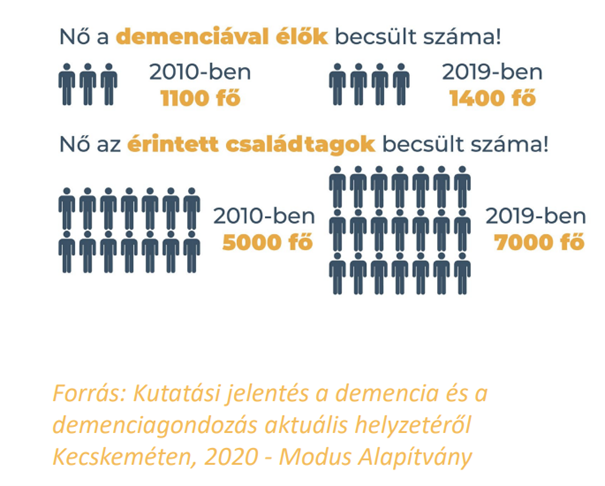
\includegraphics[scale=0.7]{images/demencia.png}
		\caption{Valamely demenciafajtával diagnosztizáltak számának emelkedése}
		\label{fig:demencia}
	\end{figure}

	Az értelmi hanyatlást különféle egészségkárosító szokások -- például az alkoholfogyasztás -- szervi károsodás, akár ezek együttese is okozhatja, a legjelentősebb kockázati tényező ilyen téren azonban az ember életkora. 
	%todo: FORRÁSOK!
	
	Szakemberek véleménye szerint a megfelelő étrendek megalkotásával, a társas interakciók intenzitásának és tartalmi színvonalának növelésével, az emberek képzésével mind iskolai, mind munkahelyi szinten megelőzhetjük agyi teljesítőképességünk romlását. 
	Kifejezetten preventív jelleggel hatnak a különféle társasjátékok, valamint a rejtvényfejtés.\\Egy szó, mint száz: bármi, amivel munkára bírjuk agyunkat, alkalmas arra, hogy gátat vessen annak romlásának.
	Végül és abszolút nem utolsó sorban említhetjük a mozgás fontosságát, munkánkban a demencia megfékezésének ezen útját választottuk.

	Szakdolgozatom ezen pontján azért érdemes erről a betegségről szót ejtenem, mivel alapvetően számomra már önmagában motivációul szolgál a tudat, hogy egy ilyen nagy volumenű elmélet megvalósításában vehetek részt, amely a demencia megelőzését, a mentális állapot folyamatos rongálódásának megfékezését célozza. 
	\cite{dementia1}
	\cite{dementia2}
	\cite{dementia3}

	Az általunk készített szoftver támogatást nyújthat csoportfoglalkozásokon, tulajdonképpen egy tornaórát le tudunk vezényelni az eszközöknek köszönhetően. Természetesen az eszközök által kibocsájtott különböző fény- és hangjelzések önmagukban nem hordoznak semmiféle jelentést, a jelzések konkrét  a tornaórákat vezénylő szakemberek dolga közölni a csoport számára.
	
	Bevezetésem ezen részén szeretném egy kicsit górcső alá venni témám címét. Ehhez először is meg kell ismerkednünk a címben szereplő két programozási paradigmával\\
 	Az imperatív\footnote{\textit{imperare} latin szóból eredetű szó, jelentése: parancsol} programozási paradigma arról szól, hogy a számítógépet egyértelműen, előre meghatározott utasításkészlettel vezéreljük, le kell írnunk a problémát megoldó lépéssorozatot, algoritmust, így az elkészült forráskódot ilyen lépéssorozatok együttese teszi ki. Az algoritmusok implementálásához változókat és vezérlési szerkezeteket (elágazás, ciklus és szekvencia) használunk. Az efféle megközelítést támogató nyelveket nevezzük imperatívnak. Ilyenek például a Java, a C, C++, C\# és a Delphi.
 	\\
 	Az objektum-orientált programozási paradigma igyekszik a világot lemodellezni olyan formában, hogy a modellt objektumok használatával írja le. Az OOP egyik alaptézise, hogy az adatszerkezet és a rajtuk végzett műveletek egy egységben, az osztályban összpontosulnak. Az osztály a belőle készíthető objektumok ,,tervrajzának'' nevezhető. Ennek megfelelően egy osztályba tartoznak a változók és a rajtuk végrehajtható metódusok. Változóinkat és metódusainkat védettségi szintekkel láthatjuk el, hogy a hozzáférést bizonyos erőforrásokhoz korlátozzuk, ellenőrzött módon végezzük. Az osztályok között kapcsolatokat teremthetünk: öröklődést vagy birtoklást. Azon nyelvet, amelyek ezt a paradigmát támogatják, objektum-orientáltnak minősítjük.
 	A fentebb említett nyelvek ezt a paradigmát is támogatják a C nyelv kivételével.
	\chapter{Programozási nyelvekről általában}
	\section{A programozási nyelvek formális nyelvek?}
	\begin{definicio}
		Legyen $\mathbb{A} = \{a_1, a_2, ... a_n\}$ véges, nemüres ($ \mathbb{A} \neq \emptyset$) halmaz, ezt a nyelv ábécéjének, elemeit betűknek vagy jeleknek nevezzük. $\mathbb{A}$ halmaz elemeiből képezzük annak hatványait, ekkor 
		\begin{enumerate}
			\item $\mathbb{A} ^ {0}$ az üres szó ($\epsilon$) egyelemű halmazát, 
			\item $\mathbb{A} ^ {1} $ az egybetűs szavak (\,$\mathbb{A}^{1}\subseteq\mathbb{A}\wedge\mathbb{A}\subseteq\mathbb{A}^{1} \iff \mathbb{A}^{1}=\mathbb{A}$\,), 
			\item $\mathbb{A}^{2}$ a kétbetűs szavak, 
			\item $\mathbb{A}^{n}$ az $n$ hosszú szavak halmazát jelenti és így tovább.
		\end{enumerate}
	Jelölje $A^{*}=A^{0}\ \cup\ A^{1}\ \cup\ A^{2}\ \cup\ \dots\ \cup\  A^{n}$ az ábécé elemeiből képzett véges szavak vagy más néven jelsorozatok halmazát (ezt az $\mathbb{A}$ ábécé feletti univerzumnak hívjuk). Ekkor  $\mathbb{A}$-ból kirakható szavak $\mathbb{A}^{*}$ halmazának egy részhalmazát \textbf{formális nyelvnek} nevezzük. Szokásos még az $\mathbb{A}$ ábécé feletti formális nyelv megnevezés is. A hatványok a halmaz önmagával vett \emph{Descartes-szorzatait} jelentik.
	\cite{formnyelvek}
	\end{definicio}
	
	Fő különbségek formális és természetes nyelvek között:
	\begin{itemize}
		\item A formális nyelveket egy dedikált célra hozzuk létre, ezeket általában nem használjuk interperszonális (emberek közötti) kommunikációra. Ezzel szemben egy természetes nyelv (például az angol) egy emberi közösség aktuális és a múltban használt jelkészletét rendszerezi.\\
		A C++ programozási nyelv például azért jöhetett létre \textit{Bjarne Stroustrup} dán szoftverfejlesztő jóvoltából, mert a C - procedurális paradigmájú nyelv lévén - nem tette lehetővé többek között a tisztább objektum-orientált programozást, a memóriacímek helyett a biztonságosabb referenciák használatát. \cite{cpplang1}
		\item A formális nyelvek kulcsszavakból állnak. A természetes nyelvek több építőelemből tevődnek össze: fonémák (hangok, betűk), morfémák (szótövek, toldalékok), szavak, mondatok, bekezdések, szövegek.
		\item A természetes nyelvek fejlődhetnek spontán, emberi generációról generációra valamint tudatos módon (például nyelvújítás) egyaránt. A formális nyelvek alakulását egy tervezési fázis előzi meg, ekkor a nyelv szabályrendszerét lefektetik, tehát csak és kizárólag tudatos, mesterséges beavatkozással lehet megreformálni őket.
		\item Az ember által is beszélt természetes nyelvek esetén a használt szavak hangsúlyozásának, hanglejtésének, valamint a beszéd hangerejének is jelentésmódosító ereje lehet, a formális nyelvek esetében hangsúlyról egyáltalán nem beszélhetünk.
	\end{itemize} \cite{langvid1} \cite{langvid2}
	Ezekből következően minden programozási nyelv formális nyelvnek számít.
	\section{Jelenleg népszerű programozási nyelvek}
	2022-ben a legnépszerűbb programozási nyelveknek számítanak (a teljesség igénye nélkül):\cite{proglanguages1}\cite{proglanguages2}
	\begin{enumerate}
		\item \textbf{JavaScript}
		\begin{itemize}
			\item 1995, \textit{Brendan Eich} fejlesztette a webböngészési funkcionalitások kibővítése végett.
			\item web-, játék-, valamint mobilfejlesztésre egyaránt használják
			\item webszerverként is tud funkcionálni (Node.js)
		\end{itemize}
		\item \textbf{Python}
		\begin{itemize}
			\item 1991, \textit{Guido Van Rossum} tervezte annak érdekében, hogy olvashatóbb és nagyobb kifejezőerővel rendelkező kódok készülhessenek, a szintaktikai szabályok helyett a kód működésére tudjanak a programozók koncentrálni
			\item backend-fejlesztés
			\item automatizálás
			\item web scraping\footnote{Információgyűjtés eszköze, amely lehetővé teszi, hogy automatizált módon (kód segítségével) bizonyos weboldalakról tetszőleges adatokat (például posztokat, közelgő eseményeket) letölteni.}
			\item Data Science\footnote{Az informatika, a matematikai statisztika és az üzleti elemzés metszetében álló tudományág, amely adatok összegyűjtésével, ezek elemzésével foglalkozik annak érdekében, hogy a vállalatok jobb üzleti döntéseket tudjanak meghozni ezek segítségével. Forrás: \cite{q_datascience}}
		\end{itemize}
		\item \textbf{HTML}
		\begin{itemize}
			\item webdokumentumok kezelése: JSON, XML, SVG
			\item weboldalak statikus (állandó) részeinek fejlesztése
		\end{itemize}
		\item \textbf{CSS} 
		\begin{itemize}
			\item weboldalak formatervét, kinézetét, stílusát alakítja ki
			\item HTML mellett hívják segítségül
		\end{itemize}
		\item \textbf{Java}
		\begin{itemize}
			\item 1995, Sun Microsystems fejlesztése, alapötlet: olyan eszközök vezérlése, amelyek elférnek egy kézben
			\item E-kereskedelem
			\item Financial Technology: pénzintézetekkel, tőzsdékkel, számlázással kapcsolatos szoftvereket jellemzően ezen a nyelven fejlesztik
			\item a megírt kódok futtathatóak különösebb átalakítás nélkül az elterjedtebb operációs rendszereken (a kód hordozható, platformfüggetlen)\footnote{Ez azért lehetséges, mivel .exe fájl helyett egy átmeneti .class állomány (bytecode) készül, amit egy virtuális gép (Java Virtual Machine) tolmácsolja (interpretálja) gépi kódként a számítógépünknek
			Forrás: \cite{jvm}}
		\end{itemize}
		\item \textbf{SQL}
		\begin{itemize}
			\item 1972, \textit{Donald D. Chamberlin} és \textit{Raymond F. Boyce} az IBM alkalmazásában, adattáblák egyszerűbb kezelésének érdekében hozták létre
			\item adatbázisok kezelése, karbantartása
			\item Data Science
		\end{itemize}
		\item \textbf{Go}
		\begin{itemize}
			\item 2009, a Google fejlesztői alakították ki, hogy megoldják a hatalmas szoftverrendszerekkel kapcsolatos problémákat
			\item rendszerek, hálózatok programozása
			\item hang- és videószerkesztés
			\item Big Data\footnote{Az informatika egyik tudományága, amely tömérdek mennyiségű, hagyományos számítógéppel nehezen kezelhető adatok tárolásával és feldolgozásával, ezek elemzésével foglalkozik.
			Forrás: \cite{bigdata}}
		\end{itemize}
		\item \textbf{C}
		\begin{itemize}
			\item 1970-es években Ken Thompson és Dennis Ritchie jóvoltából, Assembly-nél magasabb szintű (természetes nyelvezethez közelebb álló) nyelv kialakítása volt a célja
			\item hardverelemek illesztőprogramjai, vezérlőkódjai
			\item operációs rendszerek fejlesztése
			\item 3D videók szerkesztése
			\item alacsonyabb szintű a fentebb felsoroltaknál, ezért könnyebb optimalizálni memória és futásidő szempontjából
			\cite{clang1}
		\end{itemize}
	\end{enumerate}
	Összességében elmondható, hogy a programozási nyelvek eszközökként szolgálnak a fejlesztők kezében. Véleményem szerint minél több eszközt ismerünk, annál jobban meg tudjuk határozni, hogy az előttünk álló problémához az eszköztárunkból melyik lenne a legalkalmasabb, amellyel kényelmesen és hatékonyan tudunk dolgozni.
	\section{Milyen adatszerkezeteink vannak?}
	A programozási nyelvek szintaktikában ugyan eltérnek egymástól, amikor viszont adatok tárolásáról van szó, egy dologban egyetértenek: típusokra szükség van. Mit jelent az, hogy egy változót például \verb*|bool| típusúként definiálunk? Az adat típusa meghatározza, hogy
	\begin{itemize}
		\item mekkora memóriaterületet\footnote{A memóriaterület mértékegysége alapértelmezetten bájtban értendő, mivel 1 bájt számít a legkisebb megcímezhető memóriaegységnek.} kell számára lefoglalni
		\item a számítások folyamán hogyan kell őt értelmezni\\(például ha másik változónak értékül adjuk, hány bitet kell másolni)
		\item továbbá milyen műveletek végezhetőek vele\\(például egész típusú változókon értelmezhetjük a szorzás műveletét, szövegeknél ezt már nem tehetjük meg).\cite{adatszerkezetek_88}
	\end{itemize}
	\section{Használt adatszerkezetek}
	Ahogy említettem, a programozási nyelvek döntő része típusos, ezenfelül kisebb-nagyobb különbséggel hasonló adatszerkezeteket értelmez.
	\begin{enumerate}[label=\alph*)]
		\item \emph{elemi adattípusok}: Elemi/primitív típusokat nem tudunk további részekre bontani, csak egyben értelmezhetjük őket. Ilyen például a \verb*|double| lebegőpontos típus, amely 8 bájton képes lebegőpontos számot ábrázolni. Igaz, hogy csak az első bájtra van mutatónk, de nincs értelme további bájtokra darabolni, és megnézni az értékeket, mivel egyben értelmezendő, a műveleteket 4 byte-on fogjuk tudni vele végezni. Primitív adattípusoknak is nevezzük őket.\\
		Vegyük például a C\# programozási nyelvet, milyen elemi típusai vannak?
		\begin{enumerate}
			\item egész:
			\begin{tabular}{ccc}
				Előjeles típus & Előjel nélküli típus & Méret (bájt) \\
				sbyte & byte & 1 \\
				short & ushort & 2 \\
				int & uint & 4 \\
				long & ulong & 8 \\
			\end{tabular}
			\item lebegőpontos:
			\begin{tabular}{cc}
				Típus neve & Típus mérete (Bájt) \\
				float & 4 \\
				double & 8
			\end{tabular}
			\item logikai: 
			\begin{tabular}{cc}
				bool & 1 Bájt
			\end{tabular}
			\item karakteres: 
			\begin{tabular}{cc}
				char & karakterkódolástól függ\footnote{ASCII-kódolás esetén egyetlen karakter 7, míg UTF-8 kódolás esetében 8 biten tárolódik. Mivel a legkisebb megcímezhető egység az 1 bájt, ezért ezek 1 bájt területet foglalnak karakterenként, ASCII-kód esetében a 8. bit értékét nem veszik figyelembe. 
					Ezzel szemben az újabb UTF-16- és UTF-32-szabványok esetében az előbbiben 2 bájt, utóbbiban 4 bájt memóriaterület szimbolizál egyetlen karaktert. Forrás:\cite{gfg_charcoding}}
			\end{tabular}
		\end{enumerate}
		\item \emph{összetett adattípusok}: Az összetett adattípusok elemi típusokra szedhetők szét, vagyis primitív és/vagy további összetett típusú változókból épülnek fel. Ami a adattagok vagy mezőnek nevezzük. Az összetett adattípusú változók tárolásához szükséges memóriaterület kiszámítható az adattagjainak összegével.\\
		C\#-ban a \verb*|struct| és a \verb*|class| kulcsszavakkal tudunk összetett típusokat definiálni.
	\end{enumerate}
	\section{Mi a helyzet az algoritmusokkal?}
	Adatokat tudunk tárolni, és ezt tesszük azért, mert tervünk van velük, azaz valamit szeretnénk velük kezdeni. Az adatszerkezeteken végzett véges számú elemi lépéssorozatot algoritmusnak nevezzük. Az adatszerkezetek algoritmusok nélkül lényegében olyanok, mint a matematikai műveletek operátorok (összeadás, kivonás, stb.) nélkül, végül -- ha már említettem a természetes nyelveket-- mint a főnevek igék nélkül.

	
	\chapter{Marshalling}
	\section{Kommunikáció adatszerkezeteken keresztül}
	A \emph{Marshalling} egy olyan folyamat, amely összetett típusok átalakítására szolgál, hogy egy nyelv adatszerkezetét a másikkal megértessük. Magyar fordításával nem találkoztam ennek a kifejezésnek, de leginkább talán az 'átalakítás' szóval tudjuk leírni, ami adatszerkezetek esetében annyit tesz, hogy más nyelv által is értelmezhetővé tesszük, kevésbé hagyatkozunk az adott nyelv különlegességeire.\cite{sof_marshalling}
	\par
	A kód további portolhatósága, újrahasznosíthatósága végett megéri szabványos formátumokon keresztül kommunikálni, mint azt tesszük API-k\footnote{Az Application Programming Interface utasítások, szabványok és metódusok halmaza, amely leírja a kommunikációt más, külső szoftverek részére. Az API-k lehetőséget biztosítanak két vagy több szoftver közötti adatok cseréjére, valamint adatokon végzett műveletek végrehajtására úgy, hogy annak mikéntjéről az API írója gondoskodik. Másként fogalmazva: az API a szerver azon része, amely felelős a kérések feldolgozásáért és kiszolgálásáért. Forrás: \cite{api}} vagy konfigurációs fájlok esetében, ilyenek például az általam használt JSON- vagy XML-formátumok,  hogy más felületekre való költöztetés esetén kompatibilitási probléma többé már ne merülhessen fel.

	A Marshalling primitív típusok esetén abszolút működőképes, összetett adatszerkezetekre viszont inkább a szabványos szöveges formátumokat érdemes alkalmazni tapasztalatom szerint. Ha ezt elfogadjuk, akkor fontos, hogy a szerializáció és deszerializáció folyamataiba is betekintést nyerjünk.
	\section{Szerializáció}
	%todo: szerializáció - deszerializáció kifejteni
	\cite{sof_serialization}
	\section{Marshalling és szerializáció}
		A Marshalling egy olyan folyamat, amely hidat teremt a felügyelt és felügyelet nélküli kódok között, lásd: \ref{managed_unmanaged}. A Marshalling felelős az üzenetek átviteléért managed környezetből unmanaged környezetbe, és ugyanezért visszafelé is. Ez a CLR egyik alapvető szolgáltatása. Mivel az unmanaged típusok közül soknak nincs is párja a managed környezetben, így létre kell hozni konvertáló függvényeket, amelyek oda és vissza átalakítást végeznek az üzeneteken. Ennek megvalósított folyamatát nevezzünk Marshallingnak.
		\cite{marshalling_serialization}
	\section{Adatok konvertálása}
	\subsection{Egész és valós számok, logikai változók}
	Egyszerű adattípusok azok, amelyek nem tartalmaznak más adattípusokat. Ezek az alapjai minden más típusnak. Példák a menedzselt primitív szám típusokra: \verb*|System.Byte|, \verb*|System.Int32|, \verb*|System.UInt32|, és \verb*|System.Double|.
	Összetett adattípusok, amelyek más adattípusokból épülnek fel. Például egy osztály vagy egy struktúra, amelyek magukban foglalnak egyszerű vagy egyéb összetett típusokat.
	\cite{marsh}
	\subsection{Szövegek}
		%todo
		A szöveges nem menedzselt típusok Marshalling-folyamata bonyolultabb, mint a numerikusoké, mert ezek különleges kezelést igényelnek. Az alább táblázat röviden mutatja a felügyelet nélküli szöveges adattípusokat.
		
		Az ANSI és az Unicode két olyan karakterkódolás, amelyet a maguk idejében széles körben használtak. Az ANSI nagyon régi, és olyan operációs rendszerekben használják, mint a Windows 95/98, míg az Unicode egy újabb kódolás, amelyet minden modern operációs rendszerben használnak, ezért használják. A fő különbség az, hogy az ANSI-nek számos korlátja van, amelyek nem voltak nyilvánvalóak, amikor először használták, de fájdalmasan nyilvánvalóvá váltak, ahogy a számítógépek világszerte elterjedtek.
		
		Az ANSI legnagyobb hátránya, hogy a használt nyelvtől függően több kódtáblát használ, amelyek közül néhány megfelel az angol (Nyugat-Európában latin néven ismert), a görög, a török, a héber, az arab és sok más nyelvnek. Ha az adatokhoz hozzáférő összes számítógép ugyanazt a kódlapot használja, akkor nincsenek problémák, de ha különböző kódlapokat használnak, akkor az olvasott és írt adatok nem fognak egyezni. Ez adatrongáláshoz és bizonyos esetekben programhibához vezethet.
		
		Az ANSI-t nem lehet adaptálni, mert csak nyolc bitet használ minden egyes kódpont ábrázolására. Ez a szélesség rögzített, és összesen csak 256 kombináció lehetséges. Ezzel szemben a Unicode akár 32 bitet is használ minden egyes kódpontra, és az UTF-32 is fix szélességet használ. A karakterenkénti négy bájt használata azonban nagyon pazarló, ezért az UTF-8 és az UTF-16 változó szélességű kódolást használ a helytakarékosság érdekében.
		
		Mivel a Unicode egy új szabvány, várhatóan nem támogatott a régebbi operációs rendszerekben; bár az UTF-8 és az ANSI kódpontok közel azonosak, nem lehet őket régebbi operációs rendszerekben, például a Windows 95-ben működésre bírni. Ezért a Unicode-ot használó programok nem fognak megfelelően működni ezeken az operációs rendszereken. Ezzel szemben az ANSI programok futtathatók az újabb operációs rendszereken, mivel létezik egy konverziós mechanizmus az ANSI és a Unicode között. Csak azzal kell tisztában lenni, hogy ez a konverzió némi további feldolgozási többletköltséget jelent. Lehet, hogy a modern számítógépeken ez nem olyan fontos, de a program hatékonyságának növelése érdekében mégis figyelembe kell vennie.
		
		Következtetés.
		
		1. Az ANSI egy nagyon régi karakterkód, és az Unicode ma már a szabvány.
		2.Az ANSI különböző oldalakat használ a különböző nyelvekhez, míg az Unicode nem.
		3.Az ANSI fix szélességű kódolást használ, a Unicode pedig fix és változó szélességű kódolást egyaránt.
		4.A Unicode programok nem működnek a régebbi rendszereken.
		5.Az ANSI programok lassabbak, mint a Unicode programok a modern számítógépeken. \cite{ansi_unicode}
		
		A Platform invoke másolja a string paramétereket, szükség esetén a .NET Framework formátumból (Unicode) a nem kezelt formátumba (ANSI) konvertálja őket. Mivel a kezelt karakterláncok megváltoztathatatlanok, a platform invoke nem másolja vissza őket a nem kezelt memóriából a kezelt memóriába, amikor a függvény visszatér.
		
		A következő táblázat felsorolja a karakterláncok marshalling-opcióit, leírja használatukat, és linket ad a megfelelő .NET Framework-mintához.
		Mind a System.String, mind a System.Text.StringBuilder osztályok hasonlóan viselkednek.
		
		A karakterláncok COM-stílusú BSTR-típusként vagy nullvégű karakterláncként (null karakterrel végződő karaktersorozat) marshallolhatók. A karakterláncban lévő karaktereket Unicode (a Windows rendszereken alapértelmezett) vagy ANSI kódként lehet átvinni.
		
		Interfészekben használt karakterláncok
		A következő táblázat a string adattípus marshalling lehetőségeit mutatja be, amikor nem kezelt kódhoz metódusargumentumként marshallingolják. A MarshalAsAttribute attribútum több UnmanagedType felsorolási értéket biztosít a karakterláncok COM-interfészekbe történő marshalozásához.
		
		Enumerációs típus A nem kezelt formátum leírása
		UnmanagedType.BStr (alapértelmezett) Egy COM-stílusú BSTR, előre meghatározott hosszúsággal és Unicode karakterkódolással.
		UnmanagedType.LPStr Egy mutató egy ANSI karakterekből álló nullvégű tömbre.
		UnmanagedType.LPWStr Unicode karakterek nullvégű tömbjére mutató mutató.
		Ez a táblázat a Stringre vonatkozik. A StringBuilder esetében csak az UnmanagedType.LPStr és az UnmanagedType.LPWStr opciók engedélyezettek.
		
		A következő példa az IStringWorker interfészben deklarált stringeket mutatja.
		\cite{marshalling_strings}
	\subsection{Rekordok}
	\section{Managed és unmanaged kód közötti különbség}
	\label{managed_unmanaged}
	Először is fontos tisztázni, hogy a C\# szemszögéből nézve a \textit{Unmanaged Code} (nem felügyelt kód) elnevezést a .NET-keretrendszer mindenféle külső komponens megbélyegzésére használja, amelyet nem a .NET futtatókörnyezete felügyel és vezérel. Ettől még ezek lehetnek jó kódok, csak szimplán a Common Language Runtimenak nincs közvetlen hatása ezek működésére: a memóriacímeket közvetlenül lehet kezelni, felülírni, így bizonyos esetekben olyan memóriaterületre is hivatkozhat egy változó, amelyet az operációs rendszer nem a program részére foglalt le, ezt \verb*|segfault|nak nevezzük\footnote{Másnéven \textit{access violation} hibának is nevezik, a Delphi inkább ezzel a kifejezéssel él a hiba kijelzésekor.}
	\cite{managed} 
	A Common Language Runtime használatával fejlesztett kódot kezelt vagy felügyelt -- managed -- kódnak nevezzük. Más szóval, ez az a kód, amely a .NET futtatókörnyezete által végrehajtásra kerül. 
	A menedzselt kód futási környezete számos szolgáltatást nyújt a programozó számára: ilyen a kivételkezelés, típusok ellenőrzése, a memória lefoglalása és felszabadítása, így a Garbage Collection\footnote{A Garbage Collection, azaz szemétgyűjtés egy automatikusan végbemenő optimalizálási folyamat, amely során futásidő közben felszabadulnak olyan memóriaterületek, amelyek a kód korábbi részén lefoglalásra kerültek, azonban a program későbbi szakaszban már egyáltalán nem történik hivatkozás rájuk.}, és így tovább. A fent említett szolgáltatások a fejlesztőket szolgálják, hogy biztonságosabb és optimálisabb kódot készíthessenek.
	\cite{marshalling_serialization}

	A felügyelet nélküli kód ennek pontosan az ellentéte: pointereket kezelhetünk a kódban, ezeket tetszésünk szerint lefoglalhatjuk, felszabadíthatjuk, megváltoztathatjuk a pointer értékét (azaz más területre mutathatunk), viszont ilyen típusú kódok növelhetik alkalmazásaink teljesítményét, mivel az extra ellenőrzések ki vannak kapcsolva a kód lefutásának idejére (például egy tömb túlindexelését vizsgáló algoritmus).
	A nem biztonságos blokkokat tartalmazó kódot az \verb*|AllowUnsafeBlocks| fordítói opcióval kell lefordítani.
	
	Amikor eszközöket vezérlő kódrészleteket szeretnénk C\#-on keresztül hívni, legyen ez C++ vagy éppen esetünkben Delphi nyelven készítve, egyszerűen megkerülhetetlen a felügyelet nélküli kódok futtatása, mivel a C\#-nak ezekre ráhatásai nincsenek, nyelvi korlátokba ütköznénk, ha lámpákat és nyilakat kéne vezérelnünk C\#-forráskóddal. A .NET úgy áll ezekhez a kódokhoz, hogy ,,megengedett, de nem ajánlott'' kategóriába sorolja őket, nekünk annyit kell tennünk az ügy érdekében, hogy minél kevesebbszer hagyatkozzunk az unmanaged kódrészletekre.
	\cite{sof_managed}
	\section{Az ellenőrzött kódok előnyei és hátrányai}
	\begin{itemize}
		\item A futtatott kód biztonságosabb, erről ellenőrző algoritmusok gondoskodnak (például ilyen az \textit{array boundaries check}, ami a tömbök túlindexelését vizsgálja).
		\item A szemétgyűjtés automatikusan lezajlik, ezért nem is kell memóriaszivárgástól tartanunk.
		\item A dinamikus, azaz futásidejű típusellenőrzés biztosítva van.
	\end{itemize}
	
	Átokként és áldásként is felróható, hogy nem enged direkt ráhatást memóriacímekre: hogy a lefoglalások és felszabadítások mikor, a szekvenciának mely pontjain történnek meg, arról nem tudunk konkrét információkat, mivel a Garbage Collector ezt elrejti előlünk, a program bizonyos pontjain csak sürgetni tudjuk, hogy az optimalizálást előbb végezze el. 
	
	Ami ténylegesen hátrányként említhető, hogy nem enged hozzáférést alacsonyabb szintű részletekhez, így különböző mikrokontrollerek, hardverelemek vezérlésének szemszögéből kiindulva a programozás ezen módja nem tekinthető opciónak.
	\section{A Platform Invoke működése}
	A managed és unmanaged kódok közötti adattovábbítást az úgynevezett Platform Invoke (röviden PInvoke) végzi. A PInvoke-keretrendszer a projekt szempontjából egy fekete doboznak (black box) számít, mivel nem ismerjük ennek megvalósítási módját, ezért mindenképp érdemes körüljárnunk, hogy mi történik a háttérben, amikor a \verb*|[DLLImport]|-attribútumot rátesszük egy-egy metódus szignatúrájára.
	Induljunk ki egy konzolos alkalmazásból, amely egy felügyelet nélküli (unmanaged) Win32-eljárást hív meg:
	\begin{figure}[h!]
		\centering
		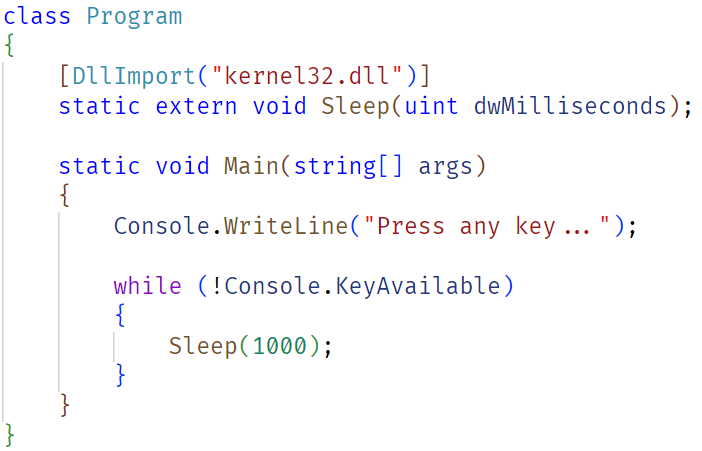
\includegraphics[scale=0.85]{pinvoke_example}
		\caption{Példa egy külsős, azaz PInvoke-eljárás definíciójára és használatára}
		\subcaption{Forrás: \cite{pinvoke}}
		\label{fig_pinvoke_example}
	\end{figure} egy Sleep-metódust, amelyet egy úgynevezett \,\textit{'kernel32.dll'}-állományban lett definiálva, meghirdetve és implementálva \ref{dll}. Ha ezt a kódot megfuttatnánk, programot két metódus írná le: az egyik a \verb*|Program.Main|\footnote{A Program.Main a program belépési pontja C\# esetében, innentől kezdődik elkészített kódjaink futtatása Lényegében ha a futtatást mappákra vetítenénk le, ő számítana a gyökérkönyvtár (root directory), amiből nyílhatnak további könyvtárak.}, a másik a \verb*|Program.Main| törzsében meghívott DLL-ből érkező \verb*|Sleep|-eljárás, mindkettő IL-kódra fordul.
	
	A .NET-keretrendszer 4-es verziója óta (projektünkben 4.7.2-es verziót használtam a DLL elkészítésére) minden PInvoke-kal hívott metódust köztes nyelvre fordítanak, és Just in Time kerül lefordításra a processzor-specifikus futtatható kódra.
	
	A következő fogalmak kifejtésre szorulnak:
	\begin{enumerate}
		\item \textbf{Call Stack}: A Call Stack (hívási verem) információkat tárol a számítógépes program aktív (meghívott) függvényeiről.\footnote{Végrehajtási veremként, programveremként, vezérlő veremként, gépi veremként is találkozhatunk a fogalommal, ezek mind ugyanazon jelentéssel bírnak a fejlesztők körében.} Bár a hívási verem karbantartása fontos a legtöbb szoftver megfelelő működéséhez, a részletek nem láthatók, magas szintű programozási nyelveken ráadásul automatikusan működnek. Számos processzor utasításkészlete eltérő utasításokat tartalmaz a programverem kezelésére. Amennyiben a Call Stack üressé válik, azt mondhatjuk, hogy kiléptünk a programból, mivel a Main-függvény is visszatért hívási helyére, azaz a vezérlés az operációs rendszerhez kerül.
		\cite{callstack}
		\item \textbf{Call Frame}: Olyan adatszerkezetek, amelyek az alprogramok állapotára vonatkozó információkat tartalmazzák: változók, visszatérési típus, visszatérés címe. Minden egyes keret egy olyan függvényhívásnak felel meg, amely még nem tért vissza értékkel. Ha például egy DrawLine nevű metódus éppen fut, amelyet a DrawSquare hívta meg, akkor a Call Stack tetejére a DrawLine-metódus tulajdonságait összefoglaló hívási keret kerül. Amikor a metódus lefutott, azaz visszatért a hívás helyére, a Call Stack tetejéről törlődik a metódusnak létrehozott keret. A Call Stack tehát Call Frame elemekből épül fel.
		\cite{callstack}
		\item \textbf{CLR}: A Common Language Runtime .NET-keretrendszer futtatókörnyezete. A fejlesztett kódot, amely a CLR fordítóján megy keresztül, felügyelt (managed) kódnak nevezzük.
		\cite{clr}
		\item \textbf{Just-In-Time-fordítás}: A Just-In-Time-fordító .NET-ben a Common Language Runtime (CLR) része, amely a .NET programok végrehajtásának kezeléséért felelős, függetlenül a .NET programozási nyelvtől. A nyelvspecifikus fordító a forráskódot a köztes nyelvre alakítja át. Ezt a köztes nyelvet aztán a Just-In-Time (JIT) fordítóprogram alakítja át gépi kóddá. Ez a gépi kód specifikus arra a számítógépes környezetre, amelyen a JIT-fordító fut. Előnyei, hogy egyrészt gyorsítja a kód futtatását, másrészt segítségével platformfüggetlen C\#-kódok készíthetőek.
		\cite{jit_compiler}
	\end{enumerate}

	Amikor a CLR találkozik egy PInvoke metódussal, egy hívási keretet (Call Frame) tárol a Call Stackre (InlinedCallFrame), amely - többek között - a nem menedzselt függvény címét tartalmazza, mielőtt meghívná a tényleges.
	
	A csonk viszont lekéri ezt a a \verb*|StubHelpers.GetStubContext()| segítségével, és meghívja a nem felügyelt függvényt.
	\cite{pinvoke}
	\cite{interop_native}
	\section{Memóriakezelés az InterOp marshaller segítségével}
	Az Interop marshaller a .NET-keretrendszer egyik komponense, amely a managed adattípusok unmanaged típusokká történő konverziójáért felelős. A memóriakezelést illetően az Interop marshaller biztosítja, hogy a memória helyesen kerül lefoglalásra, és felszabadításra a konverzió folyamatában, különösen, ha nem felügyelt kóddal dolgozik.
	Amikor felügyelt objektumokat ad át nem felügyelt kódnak, az Interop az objektumot mély másolással\footnote{A mély másolás (angoul deep copy) azt jelenti, hogy objektumonként a referencia szerint tárolt mezők is klónozódnak, úgyhogy két objektum között egyáltalán nem lehet közös referencia. Ennek ellentéte a shallow copy, azaz a sekély klónozás, amelyben a tárolt objektumok memóriacíme egy az egyben átmásolásra kerül, de ekkor egy objektum ilyen típusú mezőjének változása a klónban ugyanazt a változást eredményezi.} hozza létre, hogy a nem felügyelt kód a managed objektum befolyásolása nélkül módosíthassa az objektumot. 
	
	Amikor viszont nem felügyelt objektumokat adunk át a felügyelt kód részére, az Interop marshal egy sekély másolatot hoz létre, így a felügyelt kód hozzáférhet a memóriához. Ez azt jelenti, hogy írhatja és olvashatja egyaránt ezen változók értékeit.
	
	Fontos megjegyezni, hogy a memóriakezelést az Interop Marshaller automatikusan elvégzi, így a fejlesztőknek nem kell aggódniuk memóriaszivárgás miatt. Bizonyos esetekben azonban szükség lehet a használt memória explicit módon történő felszabadítása.
	\cite{memhandling}
	\chapter{Elosztott rendszerek}
	Az elosztott rendszerek lényege, hogy van egy alkalmazás, amivel különböző kliensprogramok (ügyfelek) kommunikálhatnak, ez a szerveralkalmazás (másnéven host vagy kiszolgáló), amely legtöbb esetben egy másik számítógépen fut, amely számítógép ráadásul egy másik hálózat tagja, tehát a két gép közötti adatátvitel internetkapcsolat segítségével valósítható meg. 
	
	Az kliens és a szerver kommunikációja kétirányú: az ügyfelek többnyire kéréseket küldenek a kiszolgáló valamely erőforrásának (adatbázis) eléréséhez, a szerver is küld a kliensprogram részére üzeneteket, tájékoztatást hibaüzenetről, a végrehajtott művelet sikerességéről, annak eredményéről, és így tovább. 
	
	A szerveralkalmazás is fogadhat bizonyos adatokat a kliensektől, ezek lehetnek bejelentkezési adatok vagy éppen a felhasználó által használt kliensprogram verziószáma, elavultabb verziók esetén akár figyelmeztetheti is a felhasználót, hogy telepítse a program egy frissebb változatát. \cite{client_server}
	
	Kliens-szerver-kommunikáción alapuló alkalmazásokat különböző módokon építhetünk fel, amelyek a témám szempontjából csak annyiból fontosak, hogy például szolgáljanak programozási nyelvek közötti kapcsolatteremtés alkalmazási lehetőségeire.
	\section{Gondolataim a streamalapú kommunikációról}
	Ebben a megközelítésben a kliens és szerver kódjának nyelve megegyezik, a téma szempontjából már ez is egy tanulsággal szolgál: kell egy közös nyelv, egy szerződés a két fél között, amelytől egyik fél sem térhet el\footnote{Amennyiben valamelyik fél eltér a meghatározott szabványtól, a kommunikáció nem fog létrejönni, a kliens és a szerver nem fogja érteni egymást.}: a streamalapú kommunikáció ezt az alábbi módon valósítja meg: szövegesen eljuttatja a szerver számára a végrehajtani kívánt metódus nevét és paramétereit.
	
	Például egy kliensalkalmazásban elküldhetjük az alábbi üzenetet a streamen keresztül: \textit{"ADD|2|3"}, ezt a szerver a várakozás állapotában megkapja, rá is illeszti az üzenet első tagját -- esetünkben ez az $"ADD"$ -- az általa ismert parancsokra, és amennyiben ismeri az $"ADD"$ parancsot, meghívja rá saját $Add(int\ a,\ int\ b)$-függvényét, majd egy hasonló stream üzenetet küld vissza a kliens számára: \textit{"OK|5"}. \cite{elearning_stream}
	
	Láthatjuk, hogy van hasonlóság a küldött üzenetek között, egy szabvány, ami leírja a kommunikáció formáját. Elméletem szerint ez már önmagában nevezhető egy közös nyelvnek a kommunikációban résztvevő két fél között. 
	
	A szerver -- így a kliens is -- ismeri a következő halmaz elemeit: $$\mathbb{A} = \{"ADD", "SUB", "MUL", "DIV", "EXIT"\}$$
	Ezeket véleményem szerint bátran nevezhetjük a közös nyelv \textbf{kulcsszavainak}, (amelyek használatával a kliens a távoli számítógép implementált metódusait hívhatjuk meg), és a résztvevő feleket ezekre feltétlenül fel kell készítenünk, hogy ezen parancsok meghívási módja, tehát az üzenetküldésre használt nyelv \textbf{szintaxisa}, valamint a várható eredmény ismert legyen.
	
	Ha továbbgondoljuk, a nyelv szemantikája is megadható: tegyük fel, hogy az előbb felsorolt parancsok használatához szükség van bejelentkezésre. Bejelentkezik $$"LOGIN|username|password"$$ üzenettel a szerverre, amely eldönti, hogy a bejelentkezési adatok passzolnak-e az általa eltárolt felhasználói rekordok bármelyikével, amennyiben igen, bejelentkezteti a felhasználót a szerverre. Ekkor már a többi parancs is megnyílik a számára, a $"LOGIN"$-parancs letiltásra kerül. Ha a bejelentkezést követően a felhasználó a $$"LOGIN|username|password"$$ parancsot ismételten kiadná, kapna a szervertől egy $"ERROR|ALREADY\_LOGGED\_IN"$ üzenetet.
	 
	Szintaktikailag\footnote{\textbf{Szintaxis :} A szavak és mondatok helyességét vizsgáló tudományág. Programozásban az elgépelt kulcsszavak, azonosítók, az idézőjelek és zárójelek helytelen használata, és így tovább. A Chomsky 2-es típusú (kontextustól független) nyelvtanok leírják a legtöbb programozási nyelv szintaxisát.} ugyan helyes parancsot adott ki a felhasználó -- azaz az általa futtatott kliensprogram --, de már a parancs meghívása ebben a kontextusban (ebben a párhuzamban kontextusnak számíthatjuk a sessiont)\footnote{Egy többfelhasználós rendszerben munkamenetnek (session) nevezzük azt az időszakot, ami eltelik a felhasználó be- és kijelentkeztetése között, ekkor az szabadon végezheti a dolgát, nem kell minden egyes funkció használatához bejelentkeznie.} már egyszer megtörtént, így a megkapott hibaüzenetben tulajdonképpen egy \textit{szemantikai hibáról}\footnote{\textbf{Szemantika (jelentéstan)}: A mondatok jelentésének vizsgálata egy kontextuson belül. A programozási nyelvek terén ez azt jelenti, hogy kifejezéseket vizsgálhatunk, hogy annak az van-e értelme az adott kontextuson belül. Például amikor egy 'i' nevű változónak növeljük az értékét (\textit{i = i + 1} vagy \textit{i++}), viszont 'i' korábban nem volt definiálva, akkor \textit{szemantikai hibáról} beszélünk. A Chomsky 1-es típusú (kontextusfüggő) nyelvtanok képesek leírni a legtöbb programozási nyelv szemantikáját.} kap tájékoztatást a felhasználó. \cite{formnyelvek}
	
	\section{RESTful alkalmazások}
	A szerver-kliens-architektúrák megvalósításának egyik legnépszerűbb módja egy RESTful alkalmazás készítése. A szerver különféle erőforrásai (adatbázisban lévő táblák, az ezeket módosító függvények) különböző Unified Resource Identifiers (URI) címeken keresztül érhetőek el. A kliensnek elegendő ezen URI-címek valamelyikét meghívni, a hívással egy kérést intéz a szerver felé, majd az valamilyen szabványos szöveges formátummal -- ilyen például a JSON is -- képes visszaküldeni a kérés eredményét a kliensprogram számára.
	
	\section{Google RPC és a Proto-nyelv}
	\label{grpc}
	A Google RPC, röviden gRPC a Google jóvoltából készült nyílt forráskódú RPC-keretrendszer. Remote Procedure Callnak\footnote{magyarul: Távoli eljáráshívás} nevezzük, amikor $A$ processz meghívja $B$-nek valamely meghirdetett szolgáltatását, így $B$ a kért műveletet implementációja szerint elvégzi, majd $A$ részére visszajuttatja az általa kért művelet eredményét. Így $A$-nak nem kell törődnie a végrehajtott algoritmus részleteivel, ennek implementációja és futtatása $B$ részére delegálódik. Ez lehetőséget teremt arra, hogy bizonyos kódrészleteket, implementációkat egy másik számítógépre, egy szerverre helyezzünk át, ettől lesz a hívás ''távoli''.

	Hogy az RPC-t jobban megértsük, gondoljunk egy távirányítóra: a távirányítóval képesek vagyunk távolról vezérelni a televíziót, be- és kikapcsolhatjuk, csatornát válthatunk a segítségével, változtassunk annak hangerején, és így tovább. A távirányító a televízió azon tulajdonságait tudja elérni, amelyek számára ''meg vannak hirdetve'', azaz amely gombokra reagál a tévékészülék. A tévé által meghirdetett szolgáltatásait meg tudjuk hívni távirányítón keresztül. A ''távoli hívás'' segítségével elértük, hogy ne kelljen minden alkalommal fizikailag közel lennünk a készülékhez, amikor annak beállításain módosítani kívánunk. Ugyanakkor a távirányító használata alternatív megoldásként is szolgál olyan esetekre, amikor fizikai interakció nem vagy nehezebben kivitelezhető (például meghibásodott a nyomógomb vagy túl magasan helyezkedik el a televízió).
	
	A gRPC-t számos programozási nyelv támogatja, a teljesség igénye nélkül ezek a Java, C\#, C, C++, Kotlin, Python és PHP-nyelvek. Még Delphiben is létezik egy külső komponens, amit a projekthez hozzáadva használhatjuk a gRPC nyújtotta szolgáltatásokat. \cite{grpc_delphi}

	A keretrendszer működtetője az úgynevezett \textit{Protocol Buffers}, amely nyelv- platformfüggetlen adatcserét biztosít. A gRPC-ben ennek a segítségével teremthetünk kapcsolatot különböző vagy azonos programozási nyelven készített alkalmazásaink között, egy szerveralkalmazáshoz különféle platformokra írt kliensprogram is kapcsolódhat, mivel a kérések és válaszok nyelvezete közös, szabványos. 
	
	Ami weboldalaknál a HTML és a JSON-formátum, az a gRPC esetén a Proto-nyelv, ami átjárást biztosít akár más nyelven írt programok részére is. Amely nyelv képes implementálni a gRPC-t, a Proto-nyelvből le tudja gyártani maga forráskódját, valamint a forráskódjából is generálható a Proto-formátum, az alkalmas ezen a nyelven keresztül összekapcsolódni más, ugyanezt a keretrendszert alkalmazó szerverprogrammal is. A Proto-nyelv választott témám szempontjából kruciális, mivel kifejezetten erre a célra lett kitalálva, hogy programozási nyelvek felett álljon, ezért úgy gondolom, érdemes tovább vizsgálnunk a nyelvben rejlő lehetőségeket.

	Miért kell ehhez egy külön nyelv? Nem lehetne maradni a jól bevált JSON-nél? A Proto-nyelv további előnyökkel jár, amelyeket sem a JSON, sem az XML, sem bármilyen  más szerializált formátum nem tud biztosítani: az adatszerkezeteket szigorúan típusosan írja le.

	Ezenkívül nemcsak adatok, hanem szolgáltatások leírására is egyaránt alkalmas a Proto-nyelv, ezért is érdemes az RPC ezen változatát használni, mivel nagyobb rugalmasságot biztosít, mint egy átlagos szerializált formátum.
	\begin{figure}[h]
		\centering
		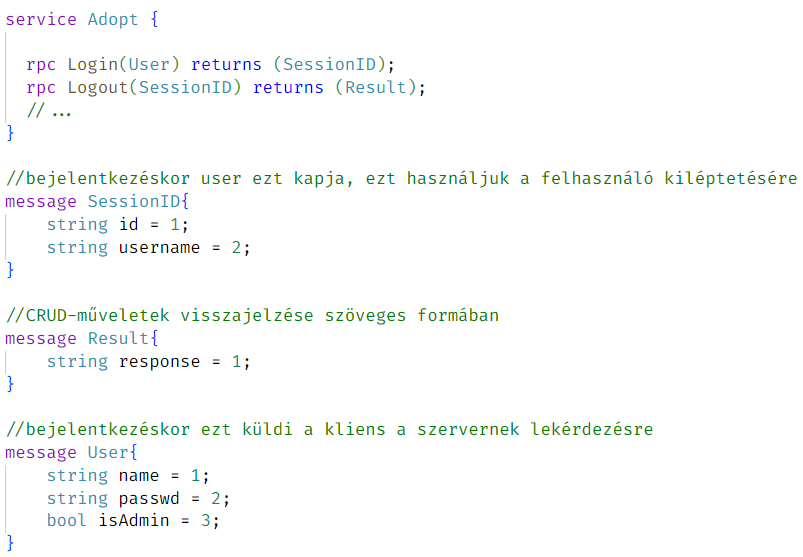
\includegraphics[scale=0.4]{protobuf}
		\caption{Beadandó projektben készített .proto állomány (részlet)}
		\label{fig:protobuf}
	\end{figure}

	Lényegében elég a fentebb látható .proto kiterjesztésű fájlt elkészítenünk, ennek környezetét, a kliens- és szerveroldali stubok forráskódjának vázát az adott nyelv szabályrendszere szerint képes lesz legyártani ebből. Ennek lehetősége a legtöbb RPC-keretrendszernél nem áll fenn.

	Mint azt említettem, Proto-nyelvben a változókat csak típussal együtt vehetünk fel\footnote{Ezen tulajdonsága miatt a Proto szigorúan típusos nyelvnek számít.}, osztályokat \verb*|message|, a meghívható metódusokat a kifejezőbb \verb*|rpc| kulcsszóval látja el. Mint láthatjuk, a mezők nevéhez 1-től kezdődően számokat rendelünk, ez a szerializációhoz szükséges. Binárisan ez úgy fog kinézni, hogy a mező azonosítóját annak típusával kombinálják, ezzel lényegében egy mező leírásához pusztán 1 bájtnyi terület elegendő. Ha üzeneteinket úgy szervezzük, hogy azonosítókat 1-től maximum 15-ig terjedően oszthatunk ki (tehát legfeljebb 15 mezőt engedünk meg osztályonként), akkor ez a tulajdonság garantált. 
	
	Természetesen ez is a gRPC előnyeihez sorolható, hogy kevesebb adatot kerül átadásra szervertől kliensig, és fordítva.
	Az adatokat a lehető legtömörebb bináris formátumban képes leírni és szállítani a hálózaton, a JSON-formátum ezzel szemben egy az egyben szövegesen kerül átadásra, ami jóval több adatforgalmat tesz ki.

	Emellett nyugodtan kijelenthetjük, hogy ez a megoldás típusbiztonsági szempontból is előnyösebb, mivel a Proto-nyelvet használva a mezőket eleve típusokkal kötjük, így nem az érkezés helyein kell validálni a megérkezett adatokat. Szöveges szerializáció esetében minden alkalommal, amikor például JSON érkezik, elsősorban ellenőriznünk kell, hogy a fogadott JSON-stringben az értékek típusai rendre megegyeznek-e az osztályban definiált mezők típusaival. Ez a Proto-nyelv esetében automatikusan teljesül, mivel a típussal kapcsolatos hibák már a küldéskor kiütköznek.
	
	Az adatokat a lehető legtömörebb bináris formátumban képes leírni és szállítani a hálózaton, a JSON-formátum ezzel szemben egy az egyben szövegesen kerül átadásra, ami jóval több adatforgalmat tesz ki. \cite{grpc_rest}
	
	GRPC-vel négyféle metódushívást tudunk leírni
	\begin{itemize}
		\item \textit{Unáris hívások}: Itt egyszerű kérés-válasz-üzeneteket cserélünk. Ez Protoban úgy néz ki, hogy a szolgáltatások paramétere és visszatérési értéke is message típusú.
		\item \textit{Kliens streamelés}: A kliens egy streamet, egy adatfolyamot (kvázi egy listát) küld paraméterben a szerver részére, a kiszolgáló pedig egy normál message-objektummal tér vissza.
		\item \textit{Szerver streamelés}: A kliens elküld egy kérést, és a szervertől válaszként streamet fogad.
		\item \textit{Kétirányú streamelés}: A kliens és a szerver is streamekben kommunikál egymással.
	\end{itemize}
	\begin{figure}[h!]
		\centering
		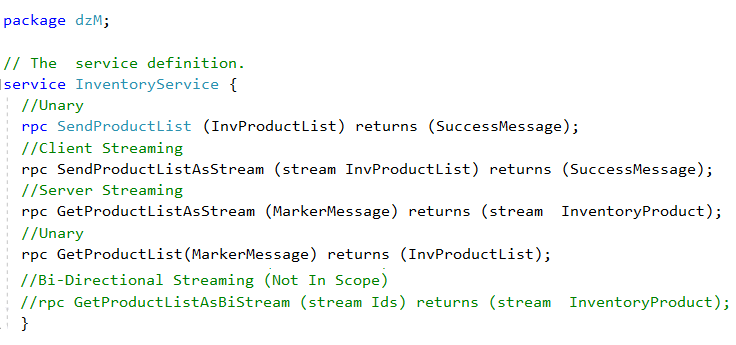
\includegraphics[scale=0.9]{grpc_calls}
		\caption{gRPC metódushívásainak típusai}
		\label{fig:grpc_calls}
	\end{figure}
	\subsection{Jobb a Proto a JSON-formátumnál?}
	Az alábbi ábrán látható, hogy a bináris szerializációt alkalmazó Proto-kérések futásidőben sokkal gyorsabbnak bizonyultak, mint a JSON-t használó REST-hívások, a kísérlet győzteseként a \textit{kliens streamelés} került ki (63.25 ezredmásodperccel), ami körülbelül 13-szor gyorsabb, mint a leglassabb REST-módszer (792.51 ms), és legalább 5-6-szor gyorsabb, mint egy átlagos REST JSON-hívásokkal. A másik két gRPC-hívás (Unáris és kötegelt\footnote{A \textit{batch}, azaz kötegelt programozásban nagy mennyiségű adatot kötegelt formában dolgozunk fel. Az adatok egy bizonyos időszakban összegyűlnek, majd ezek feldolgozása egy menetben történik. Ilyen például a bérszámfejtés, ami megvárja, hogy egy munkás munkaórái összegyűljenek a hónap során, majd a hónap lezárultát követően a megadható munkabért meghatározza. Forrás:\cite{batch}} kliens streamelt hívás 63.39 ms és 69.52 ms eredményekkel) is hasonlóan teljesítettek, és pár ezredmásodperccel maradtak le az első helyezetthez képest.
	\cite{grpc_performance}
	\begin{figure}[h!]
		\centering
		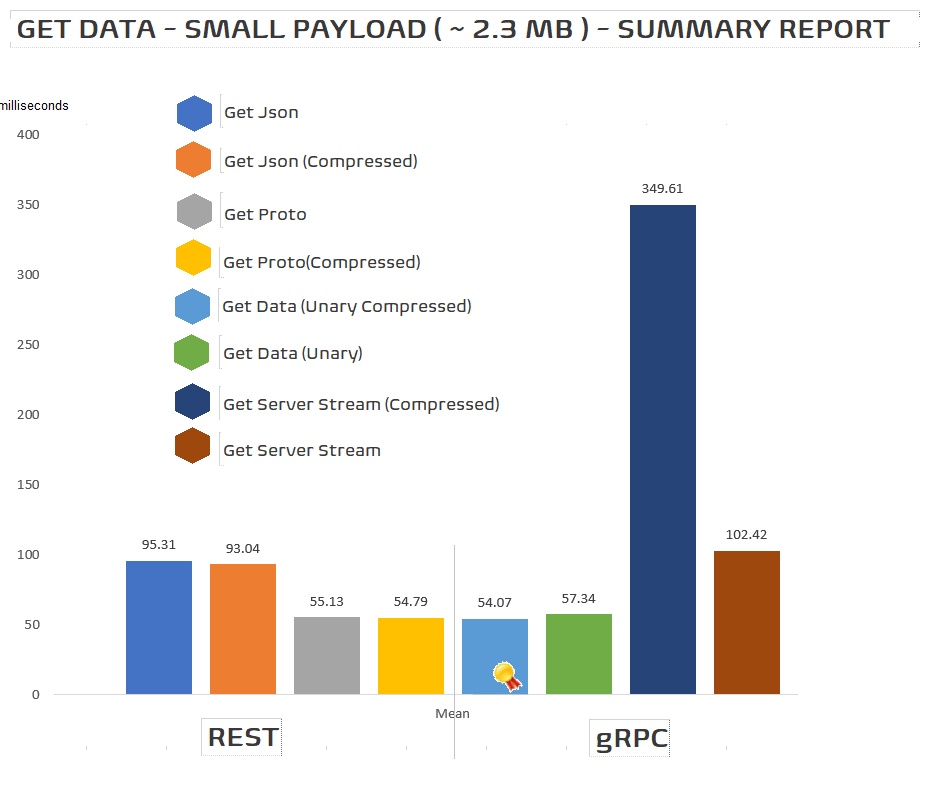
\includegraphics[scale=0.35]{grpc_json}
		\caption{Szerializáció teljesítményének összehasonlítása JSON és Proto esetében}
		\subcaption{Forrás: \cite{grpc_performance}}
		\label{fig:grpc_json}
	\end{figure}
	\chapter{Szakdolgozati projektünkről}
	Eme dokumentum mellé készített szakdolgozati szoftverprojektemet Sipos Levente hallgatótársam részére, az ő feladatának megkönnyítésének céljából készítem. 
	Munkánk arról szól, hogy Keresztes Péter tanár úr által Delphiben implementált metódusokat hívunk meg .NETes környezetből. A C\# és Delphi programozási nyelvek összehangolása az én feladatom, az elkészült termék terveim szerint úgynevezett Helper-metódusok implementációit tartalmazó, lefordított\footnote{Lévén a C\# fordított nyelvnek számít, ezért az alkalmazások futtatásához/használatához az elkészült forráskódokat első lépésben futtatható állományra (gépi kódra) kell fordítani egy fordítóprogram segítségével. Ezt a folyamatot szakszóval \textit{compilingnak} vagy \textit{buildelésnek} is nevezzük.} DLL-projekt lesz, amelyeket Levente az ő Windows Forms keretrendszerrel készített grafikus alkalmazásában tud meghívni. A projekt jelen állása szerint szükség volt továbbá egy úgynevezett relayDLL-re, amelyet én állítottam össze.

	\section{Miről is szól a projektünk?}
	Egy mentális egészségfejlesztésre használatos alkalmazást fejlesztésére vállalkoztunk 2022 szeptemberében, amely elméleti alapjait Somodi László futballedző munkásságának köszönhetjük, ezek gondolati vonulatairól titoktartási szerződésünk lévén csak nagyon érintőlegesen fogok beszámolni a későbbiekben. 
	
	A készített alkalmazásunk gyakorlatilag különböző fény- és hangjelzések kibocsátására alkalmas eszközök (lámpák, nyilak és hangszórók) vezérléséből áll, egy úgynevezett \emph{intelligens szobában} az eredeti tervek szerint 8 eszköz (a készített program azonban tetszőleges, $n$ darabszámú eszköz vezérlésére lett felkészítve) együttes vezérlését kell kezelnünk megadott időközönként, amely időközöket egyszerűen ütemnek fogjuk nevezni.
	A módszer alkalmazása az intelligens szobával együtt működik teljességében.
	
	\section{Mit jelent az intelligens szoba?}
	Az intelligens szoba elnevezés olyan helységet takar, amelynek mind a négy falán jeladókat helyeztünk el.
	Ezek különböző típusú eszközök: fények, nyilak és hangok. 
	Ezek különállóan vagy együttesen jeleket küldenek, amely jelekre speciális mozdulatokat kell a foglalkoztatottnak végrehajtani.
	Az eltérő színek más feladatokat írnak le, mást kell tenni piros, és szintén mást zöld szín felvillanása esetén, ez emlékeztetheti az embert a forgalmi jelzőlámpák működésére is: minden színhez más jelentést rendelhetünk. A nyilak felvillanásának és a hangszóróból érkező különféle hangok észlelése esetén pedig irányváltásokat kell végezni.
	
	Egy feladatsor több egymást követő ütemből áll, mely a programban azt fogja jelenti, hogy x másodperc késleltetéssel a felmért eszköz tömb elemeinek tulajdonságait (mezőit) a feladatsor aktuális ütemének megfelelően módosítjuk. Mivel minden eszközt együttesen vezérlünk, a program ütemenként az összes eszköz állapotát felül fogja írni, ezért szükségünk van egy olyan állapotra is, ami azt közli az adott eszközzel, hogy éppen semmit ne csináljon (azaz várakozzon). Ez a fényeszközök esetében egyszerűen (0,0,0) RGB-színkód\footnote{Az RGB-színkódolás egy szín leírását három komponens, vörös (\textbf{R}ed), zöld (\textbf{G}reen) és kék (\textbf{B}lue) alapszínek arányától teszi függővé.} közlését, míg hangeszköz esetén egy 0 dB hangerősségű tetszőleges frekvenciájú hangjelzés kiküldését fogja jelenteni.
	Somodi László edzővel való együttműködésünk Dr. Király Roland tanár úr jóvoltából jöhetett létre, akinek az alkalmazással kapcsolatos múltbéli tapasztalatait és  ötleteit folyamatos egyeztetések, konzultációk útján tudtuk segítségül hívni.
	\section{Delphi és C\# programozási nyelvek összehasonlítása}
	Először is érdemes leszögeznünk, hogy a továbbiakban Delphi alatt nem a fejlesztői környezetet, amely az Object Pascal nyelvvel dolgozott együtt, hanem inkább a programozási nyelvet értjük, jelenleg az Object Pascal megnevezés úgynevezett ,,umbrella term'' formájában él tovább.\footnote{Az umbrella term (magyarul gyűjtőfogalom) olyan kifejezés, amely több fogalmat rendel önmaga alá, így már fogalmak egy csoportját, kategóriáját jelenti összefoglalóan.} \cite{sof_delphi}
	A Delphi nyelv (megjelenési éve: 1986, a Borland nevű cég jóvoltából) idősebb nyelvnek számít a C\#-hoz (megjelenési éve: 2001, a Microsoft 
	jóvoltából) viszonyítva, ebből fakadóan egy stabilabb, kiforrottabb, időtállóbb eszköznek számít a programozók kezében. 
	
	Mindkét nyelv \textbf{objektumorientált}, ami azt jelenti, hogy bizonyos, logikailag összetartozó adatokat (mezőket), valamint a rajtuk végezhető műveleteket (metódusokat) egy egységbe zárunk, ezt az egységet a továbbiakban osztálynak nevezzük. Az osztály mezőit és metódusait különböző láthatósági szintekkel vértezhetjük fel, ezzel tudjuk védeni az osztályunk kritikus részeit más osztályokkal szemben. Az osztályok között akár öröklődéssel, akár objektum-összetétellel viszonyokat alakíthatunk ki.
	
	A két nyelv \textbf{erősen típusosnak} számít, mivel egy változó definiálásakor meg kell mondanunk azt is, hogy milyen típusú értékeket szeretnénk abban tárolni, a típusok már a forráskódban explicit módon megjelennek, így az adott nyelv fordítóprogramja fel van készítve a változó típusaira, amely változó hatókörén\footnote{Hatókör, illetve \textit{scope} alatt a program azon részét, kontextusát értjük, amely magába foglalja az adott változót. Ezen kontextusban vizsgálva a változó "életben van", tehát a memóriában hely van lefoglalva számára, nevére vagy memóriacímére hivatkozva értékét felülírhatjuk, kiolvashatjuk.} belül nem is változhat meg. Ahogy azt már korábban is említettem, a változó típusa meghatározza, hogy az értéket hogyan kell értelmezni a memóriában, a megadott típusnak mely műveletei vannak értelmezve, így például \verb|string| típuson nem értelmezhetünk logikai ÉS (konjunkció)-műveletet.
	
	Az elkészült kódok teljesítménye alapján is érdemes összehasonlítani a két nyelvet. Ehhez először is külön kell választanunk a fordításhoz és a futtatáshoz szükséges időt, lévén ezek fordított (nem interpretált) nyelvek, ezért ezek nem szimultán módon\footnote{nem egyidőben, nem egyszerre} történnek. A Delphi fordítóprogramja azonnal gépi kódot\footnote{A gépi kódban már az utasításokat is számok jelzik, ezen nyelv utasításkészlete már a számítógépben működő processzor típusától is erősen függ. Gépi kód az esetek nagy részében fordítóprogram eredménye, a hardverközeli vezérlőprogramok elkészítéséhez is inkább a magasabb szinten álló Assembly nyelvet használják.} készít, míg a C\# esetében első lépésben egy köztes nyelvű\footnote{A(z) (Common) Intermediate Language a .NET-keretrendszerben a magasabb absztrakciós szintű C\# és a legalacsonyabb gépi kód között ,,félúton'' helyezkedik el, ami még processzortól és operációs rendszertől független. A .NET Runtime futtatókörnyezete képes futtatni.} kód készül, amelyet a .NET virtuális gép képes futtatni. Bár fordítási időben a Delphi-kód abszolút győztesnek tekinthető -- mivel fordítóprogramja közvetlenül futtatható állományt készít --, a két nyelv segítségével készített programok futásideje közel azonos. Így megállapítható, hogy mérvadó teljesítménybeli különbséget kizárólag a fordítás folyamatában észlelhetünk.
	
	Ha ennél is tovább megyünk, akkor a C\#-nak nagy előnye származik abból a Delphivel való összevetésben, hogy aszinkron\footnote{ Az aszinkron programozás lehetővé teszi, hogy az alkalmazás egy időigényes folyamat futtatását háttérbe helyezze, így a programot futtató szál, lévén nem várakozik a válaszra, addig ugyanúgy képes a felhasználói interakciókat kiszolgálni. \cite{async}} kódolási lehetőséget is biztosít, amely felgyorsítja a végrehajtást, jobban ki tudja használni a rendelkezésre álló CPU teljesítményét. A LINQ\footnote{A \textbf{Language Integrated Query} (magyarul: nyelvbe ágyazott lekérdezés) egy gyűjtőfogalom a C\# nyelvbe épített szintaktikai elemekre, amely elemek lehetővé teszik, hogy akár lambda kifejezésként, akár SQL-szintaxishoz hasonló módon meg tudjunk fogalmazni lekérdezéseket bizonyos - iterálható, vagyis bejárható, az IEnumerable-interfészt megvalósító - szerkezetekre. Ilyen szerkezetnek minősül például a \textit{List} is.} használata \verb|yield| kulcsszóval az iterációkban biztosítja, hogy csak akkor van végrehajtva a kód, amikor ténylegesen szükség van rá (lusta kiértékelés). A delegate-ek használata szintén növelheti a C\#-kódok teljesítményét, bár a Delphi is rendelkezik ehhez hasonló funkciókkal.
	%todo: esetleg ide jöhetne egy C\# és Delphi futásidő-összehasonlítási ábra (benchmark)
	\cite{perf_comp}
	
	A fejlesztés folyamán elkészített \textbf{modulokat} a különböző programozási nyelvek eltérő megnevezéseket használnak.\footnote{Az említett példákon kívül a Java-nyelvben \textit{package}-ként, míg a Pythonban \textit{module}-ként hivatkoznak az osztályokat összegyűjtő egységre.} A vizsgált két nyelv tekintetében is ez áll fenn: a C\# \verb|namespace|, míg a Delphi \verb|unit| kifejezéssel illeti, a lényegük ugyanaz lesz: 
	\begin{enumerate}
		\item \textbf{Elnevezések}: Mivel nagy projekteknél előfordulhat, hogy két, funkciójában eltérő osztálynak ugyanazt a nevet kellene adnunk, nem tehetnénk meg, mivel a fordítóprogram nem tudná eldönteni, hogy a két változat közül éppen melyiket kívánjuk érvényesíteni. Ezt a problémát orvosoljuk például a kódok modulokra való felosztásával.
		
		\item \textbf{Egységbe zárás}: A modulok lehetővé teszik a programozók számára, hogy egy funkcionalitás végrehajtási részleteit kapszulázzák és elrejtsék. Ez azt jelenti, hogy a modulok tiszta felületet biztosítanak a funkcionalitással való interakcióhoz, miközben a mögöttes kódot elrejtik és védik a véletlen változásoktól.
		
		\item \textbf{Újrafelhasználhatóság}: A kód modulokba történő kapszulázásával a programozók olyan kódot hozhatnak létre, amely több programban is felhasználható. Ez csökkenti a fejlesztési időt és erőfeszítéseket azáltal, hogy a programozók újra felhasználhatják a már megírt és tesztelt kódot.
		
		\item \textbf{Karbantarthatóság}: Ha a kódot modulokba szervezik, könnyebb karbantartani és frissíteni, mivel az egyik modulban anélkül lehet változtatásokat végrehajtani, hogy az befolyásolná az azt használó többi modult. Ez javítja a kód karbantarthatóságát és csökkenti a hibák bevezetésének valószínűségét.
		
		\item \textbf{Moduláris felépítés}: A modulok használatával kódjainkat több kisebb, könnyebben kezelhető darabra szedhetjük szét. Ez megkönnyíti a kód megértését, és mivel a komponensek így külön fájlokban találhatóak, így a kódot szimultán módon a fejlesztőcsapat több tagja is fejlesztheti.
		
		\item \textbf{Importálhatóság}: A modul legyen beemelhető más komponensbe, ehhez szükség van egy olyan összefoglaló névre, amire hivatkozni tudunk, amikor a modult használni szeretnénk máshol is.
		
		Összességében a modulok használata a modern programozás alapja, mivel segítségükkel kódjaink a későbbiekben felhasználhatóak több helyen is, karbantartásuk gyorsabb és egyszerűbb. A programozók a programokat önálló darabokra tervezik, amelyeket meg tudnak írni, majd akár el is felejthetik egy-egy komponens belső működését, tehát hogy a problémára adott megoldás hogyan lett megoldva, elég csak azzal foglalkozniuk, hogy mi az a problémakör, amit a program ezen szelete lefed.
	\end{enumerate} \cite{delphi_basics}
	
	Ami közös még a két nyelvben, hogy a fejlesztés moduljaiból Win32-szabványnak megfelelő DLL-ek készülhetnek a segítségükkel, ezek szintén lefordított, gépi kódú állományok, amelyek más szoftver forráskódjában felhasználhatóak, lényegében így válnak futtatható állománnyá.
	
	\section{Mik azok, amelyeket a C\# tud, de a Delphi nem?}
	\begin{itemize}
		\item automatikus memóriakezelés - Garbage Collector
		\item lambda kifejezések és LINQ\footnote{A LINQ, vagyis a Language-Integrated Queries -- nyelvbe ágyazott lekérdezések -- a C\# 3.0 nyelv és keretrendszer újdonsága, amely használatával egyszerűbb szintaxissal végezhetünk tömbökön, listákon, és adatbázisokon egyaránt lekérdezéseket. A típusellenőrzést a .NET fordítási időben végzi. A lekérdezések egymásba láncolhatók, tehát egyetlen utasítással egész komplex szűréseket tudunk végezni tárolt adataink között. \cite{linq}}
		\item szerializációt csak explicit, kódolt módon tudunk végezni
	\end{itemize}
	\section{Mik azok, amelyeket a Delphi tud, de a C\# nem?}
	\begin{itemize}
		\item Assembly nyelv
		\item case insensitive
	\end{itemize}\cite{pascal_csharp}
	\section{Alaphelyzet}
	Amikor a munkát megkezdtem, rendelkezésemre állt Dr. Király Roland tanár úr által fejlesztett Delphis asztali alkalmazás, amely -- mint kiderült -- a mai napig teljes mértékben használható. Ezen alkalmazás forráskódjában követtem végig az hardvereket működtető függvények hívási sorrendjét (szekvenciáját), ezek módját és eredményeit, az esetlegesen előforduló hibaüzeneteket. 
	Ezen alkalmazás C\#-nyelvű megfelelőjének elkészítését és továbbgondolását kaptuk feladatként Leventével.
	\section{Az SLDLL-függvények bemutatása}
	A következőkben a Keresztes Péter tanár úr által Delphiben implementált metódusokat, ezek kezelésének lehetőségeit fogom részletezni.
	Általánosságban elmondható, hogy minden függvény egész típusú értékkel tér vissza, amely érték tájékoztat a lefutás eredményességéről: amennyiben a hívott metódus sikeresen (hiba, kivétel nélkül) lefutott, 0-val tér vissza, ahogy ezt egyébként az operációs rendszerek processzeinél is megszokhattuk. Ettől eltérő értékek az egyes hibatípusokat hivatottak meghatározni a Win32-szabvány\footnote{A Win32-es hibakódok szabványa szerint minden hibakódnak a $0x0000$ (decimálisan: 0) és $0xFFFFFF$ (decimálisan: $16\,777\,215$) közötti tartományban kell lennie.} keretein belül. Ezen hibakódok projektünkre vonatkozó részét az alábbi táblázatban \ref{fig:errcodes} összegyűjtöttem. \cite{errcodes}
	
	A program azzal nyit, hogy felméri az USB-porton csatlakoztatott, egymással RJ11-csatlakozókkal sorba kötött eszközöket, őket a típusának megfelelő azonosítóval látja el. Az azonosító meghatározza, hogy egy eszköz milyen típusú. 
	
	\subsection{DLL megnyitása}
	A program indulásakor elsőként lefutó \verb*|SLDLL_Open|-függvényt meghívásával elkezdhetjük az SLDLL további metódusainak használatát. Ezt érdemes automatikusan lefuttatni, ennek kezelését nem a felhasználóra bízni, mivel egyrészt elfelejtheti, másrészt felesleges, hogy a felhasználó tudjon a kötelező metódushívási sorrendről. 
	\subsection{Eszközök felmérése}
	A \verb*|SLDLL_Felmeres| folyamán az elérhető, tehát csatlakoztatott eszközök felmérése elindul. Paraméter nélküli függvény, visszatérési értéke:
	\begin{itemize}
		\item \verb*|NO_ERROR|
		\item \verb*|ERROR_DLL_INIT_FAILED|
		\item egyéb - Windows műveleti hibakódok
	\end{itemize}
	\section{Az általam készített DLL-függvények bemutatása}
	\subsection{Hibakódok}
	Az alábbi táblázatban látható hibakódokat C\#-ban a következő megfelelő, egyénileg definiált kivételekkel, és sokkal kifejezőbb üzenetekkel váltom fel:
	\begin{itemize}
		\item \verb*|Dev485Exception|: Eszközök tömbjére vonatkozó hibaüzenetek
		\item \verb*|SLDLLException|: A DLL működésével kapcsolatos hibaüzenetek
		\item \verb*|USBDisconnectedException|: Az USB-porton nem észlelhető eszköz hibaüzenete.
		%todo: újabbakat hozzáadni!
	\end{itemize}
	\begin{figure}[h!]
		\centering
		\hspace*{-0.5in}
		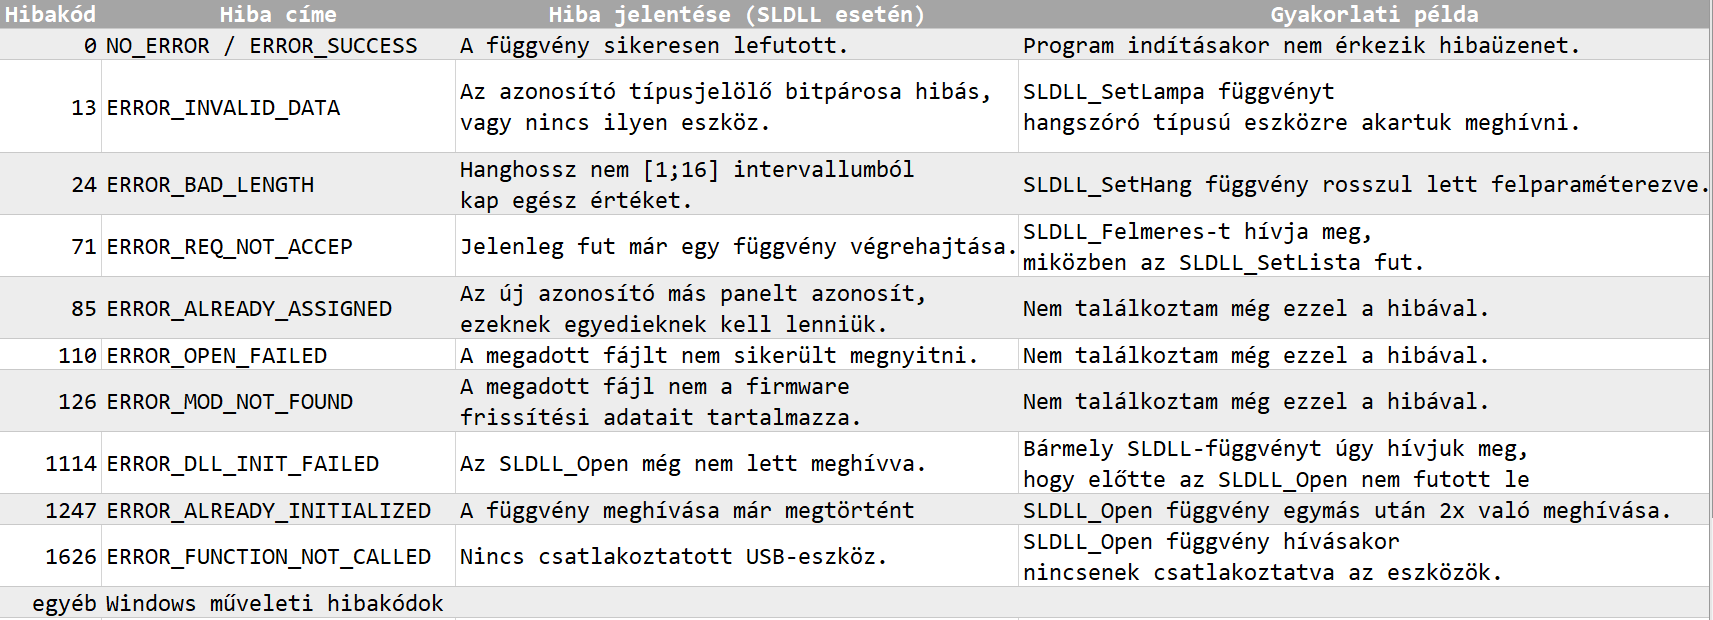
\includegraphics[scale=0.5]{images/errcodes.png}
		\caption[Hibakódok és magyarázataik]{Win32-hibakódok magyarázata}
		\subcaption{Saját szerkesztés}
		\label{fig:errcodes}
	\end{figure}
	\subsection{A WinForm bemutatása}
	A \textit{WinForm}, teljes nevén a \textit{Windows Forms} a .NET GUI-fejlesztést\footnote{A GUI a \textbf{Graphical User Interface} (grafikus felhasználói interfész) kifejezés rövidítése, asztali alkalmazásokat értünk alatta, amely átlagfelhasználók számára kényelmesebb megközelítés a konzolos alkalmazásokkal szemben} támogató keretrendszere, amelynek segítségével egy asztali alkalmazást egyszerűbb módon el tudunk készíteni. 
	
	A weblapfejlesztésből már ismert, valamint ezek tárházát bővítő vezérlőelemekkel (gombok, legördülő listák, adattáblázatok, és így tovább) gondoskodik azok újrahasznosíthatóságáról. A Visual Studio fejlesztői környezet egy Designer-felülettel is rendelkezik, amellyel gyorsan és különösebb képzelőerő nélkül elkészíthetjük grafikus alkalmazásaink vázát.
	
	Egy Windows Forms alkalmazásban a \textit{Form} (továbbiakban űrlapnak is fogom nevezni) egy vizuális felület,amely információkat jelenít meg a felhasználó számára.Egy Windows Forms alkalmazás általában úgy készíthető el, hogy egy Formhoz vezérlőelemeket (Control) adunk,a felhasználó által végrehajtott műveletekre, például egérkattintásokra és billentyűleütésekre adott válaszokat implementálunk. A \textit{vezérlőelem} különálló GUI-elemek gyűjtőfogalma, amely adatokat jelenít meg vagy adatokat fogad bevitelre.
	
	Amikor a felhasználó műveletet hajt végre egy űrlapon vagy annak vezérlőelemein, ez a művelet eseményeket generál. Az alkalmazás kódban reagálhat ezekre az eseményekre, amennyiben azok bekövetkeznek, de figyelmen kívül is hagyhatja azokat.\cite{winform}
	\subsection{DLL-ek üzenetküldése Win32-ben}
	Egy üzenetlistán\footnote{A Message Queue (üzenetsor) egy sor (queue) adatszerkezetben, érkezési sorrendben tárolja az üzeneteket, majd ezek ugyanezt a sorrendet megtartva kerülnek le róla.} keresztül kommunikál az operációs rendszer a futó programmal, ezt projektünk szempontjából Levente ablakos alkalmazása fogja jelenteni. Az operációs rendszer ráteszi a lenyomott gomb által kiváltott üzenetet erre a listára, tehát például amikor az egér bal gombjával kattintunk, akkor azt ténylegesen nem a futó program fogja észlelni, mivel az operációs rendszer a központ, ahova az I/O-kérések befutnak. 

	Az operációs rendszer eleve azért felelős, hogy elossza az erőforrásokat és kezelje a kimeneti-bemeneti perifériákat, így az egerünk által kiadott jel is az operációs rendszerhez érkezik be.
	Az alábbi lépéssorozat fog lejátszódni:
	\begin{enumerate}
		\item Az operációs rendszer ráteszi a \verb*|WM_LBUTTONDOWN|-üzenetet az üzenetsorra.
		\item A programunk meghívja a \verb*|GetMessage|-függvényt.
		\item A \verb*|GetMessage| leveszi a \verb*|WM_LBUTTONDOWN|-üzenetet az üzenetsorról, és az érkező információkból feltölti a Message-adatszerkezetet.
		\item A programunk meghívja a \verb*|TranslateMessage|- és \verb*|DispatchMessage|-függvényeket, utóbbiban az operációs rendszer meghívja az asztali alkalmazás WndProc-függvényét Ez minden esetben lezajlik, attól függetlenül, hogy az ki van-e fejtve vagy sem.
		\item Az ablakos alkalmazásban válaszolunk az I/O-kérésre (például egy gombra kattintva újabb ablakot nyitunk meg) vagy éppen figyelmen kívül is hagyhatjuk, ekkor a felhasználó belátja, hogy lényegében nem is történt semmi.
	\end{enumerate}

	Már az is Win32-üzenetet vált ki, ha szimplán mozgatjuk az egerünket, ekkor az egér új pozíciója is az üzenetben tárolásra kerül, innen és a Form előre meghatározott tulajdonságaiból (ablak pozíciója, szélessége és magassága) tudjuk detektálni például, hogy az egér az ablak területére érkezett\footnote{Erre vonatkozó esemény a MouseEnter-event Windows Forms esetében.}.

	Ha erre a felhasználói bemenetre fel van készítve a programunk által üzenetküldésre használt metódus\footnote{Egy-egy Win32-üzenet feldolgozását Windows Form asztali alkalmazás esetében a WndProc-metódus szolgálja.}, akkor az érzékeli, hogy erre az eseményre reagálnia kell, így egy másik állapotba lép. Természetesen a készített programban lehetőségünk van arra is, hogy egyszerűen ignoráljuk az operációs rendszer felől érkező üzeneteket.
	
	A felhasználó ebből az egész folyamatból csak annyit érzékelhet, hogy a lenyomott gomb hatására valami esemény történt a programban, így ő azt gondolhatja, hogy közvetlenül a program érzékelte az interakciót. Lényegében ez is történik, csak az operációs rendszer végzi az I/O-eszközökről érkező jelek feldolgozását, és erről egy Win32-üzenet formájában tájékoztatja az éppen futó asztali alkalmazást is.
	\section{Problémák és megoldások}
	Ebben az alfejezetben a következő, munkánkat időnként meg-megakasztó, kutatómunkát igénylő tényezőkről kívánok szót ejteni.
	\subsection{Egyénileg definiált típusok és struktúrák}
	A Delphis projekt erősen függ az SLDLL-ben megkívánt típusoktól, ezért a teljes kódot nem tudjuk C\#-ra átültetni.
	\subsubsection{Megoldás} 
	Erre a problémára megoldást nyújthat akár a marshalling, akár a szerializáció, mi a projektben utóbbi módszert választottuk az előző problémából levont következtetés miatt: ha stringet át tudunk adni, akkor bármilyen típust képesek vagyunk leírni szöveges formában, ezt átadva újból fel tudjuk építeni a másik nyelvben. A C\#-os objektumok példányai egy erre dedikált forrásból (JSON-formátumú szövegből) fognak értékeket kapni.

	A lényege a megoldásnak, hogy szerializálással küszöböljük ki a két nyelv közötti kompatibilitási hiányosságokat, ezért csak olyan adatokkal kommunikálunk, amelyek ismertek, feldolgozhatóak mindkét nyelv számára. Ilyenek a primitívek, az egész, lebegőpontos, logikai és szöveges típusok).
	\begin{figure}[h!]
		\centering
		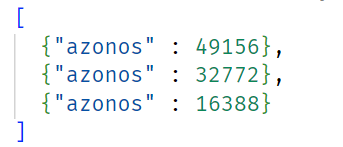
\includegraphics[scale=0.89]{json_szerializalas_azonositok}
		\caption{Eszközök azonosítóinak átadása JSON-formátumon keresztül}
		\label{json_azonositok}
	\end{figure}
	\subsection{JSON-formátumra konvertáló függvények hívása .NET keretrendszerből}
	\subsubsection{Megoldás:} A korábbi SLDLL-hez fűzzük őket, vagy tegyük egy új DLL-állományba őket, és ezeket is meg kell hirdetnünk a C\#-os futtatókörnyezet számára is. A választott megoldásom az új DLL-re esett, egy úgynevezett \verb*|relayDLL| nevezetű állomány forráskódját megírtam Delphiben, amelyen keresztül az SLDLL-függvényeket meg tudjuk hívni.
	
	Ennek legfőbb indoka az volt, ami eldöntötte, hogy érdemes a hívó (.NETben készült \verb*|FormHelperDLL|) és hívott (\verb*|SLDLL|) felek között egy köztes réteget elkészíteni, hogy Delphiben különböző globális változók kapnak értéket, amelyeket nem tudunk máshol definiálni, csakis Delphiben, tehát a hívás környezetét így tudjuk megteremteni, hogy az értékadások ténylegesen működjenek, ne fussunk \verb*|NullReferenceException|-hibákra.\\

	A \verb*|relayDLL| használatával ellenőrzöttebb módon tudom meghívni az \verb*|SLDLL|-ben meghirdetett függvényeket, ebből nem is kell mindent meghirdetni, csak annyit, amennyit ténylegesen a vezérléshez használnunk szükséges. Ezenkívül több, általam definiált hibakódot is vissza tudok adni, amelyek kiváltó okáról C\#-ban megfelelő kivételek segítségével tájékoztatni tudjuk a felhasználókat.
	\subsection{Az SLDLL\_Open-függvény paraméterezése}
	\subsubsection{A probléma leírása:} Az \verb*|SLDLL_Open|-függvény várja az ablakos alkalmazástól egy úgynevezett Handle-t, amely az üzenetküldést engedélyezi az SLDLL-függvények részéről.
	\subsubsection{Megoldás: } C\#-ban a Formnak (a függvényeket meghívó félnek) létezik egy Handle nevezetű pointere, amit átadhatunk az SLDLL-nek.
	\subsection{Stringek átadása két nyelv között}
	\subsubsection{A probléma leírása:} Különösen fontos, hogy Delphiből át tudjunk adni a Delphis relayDLL-ből a C\# részére stringeket, mivel ha ezt sikerül elérnénk, akkor bármit le tudunk írni stringként.

	Korábban szakdolgozati témánkat előkészítendő egy példaprojekt keretein belül kísérleteztem bizonyos Delphiből érkező típusok C\#-nak való átadásával. Ez természetesen kiterjedt a karakterláncokkal való kommunikációra is, mivel ha szöveget képesek vagyunk átadni, akkor lényegében segítségükkel bármilyen más típus formátuma is -- így a rekordoké is -- leírható és feldolgozható.

	Az alábbi példában vizsgáltam a referencia szerinti paraméterátadás működőképességét is, ez abban nyilvánult meg, hogy mind Delphi, mind C\# oldalon meghirdettem egy kimenő (out) paramétert, ami azt jelzi a fordító számára, hogy ez a változó az eljárás futtatásakor fog beállítódni, ennek értékét -- mivel memóriacímet adtunk át -- a függvényt hívó környezetből is el tudjuk érni. Ez különösen akkor hasznos, amikor egy függvényhívással több változó értékét is viszont szeretnénk látni.
	
	Alternatív megoldásként mindenképp érdemes megemlítenünk, hogy a visszatérési értékeket egyetlen, valami egységes karakterrel (például pontosvesszővel) elválasztva stringbe is fűzhetjük, vagy éppen egy rekordba csomagolhatjuk, ezekben az esetekben elérhetjük, hogy a ténylegesen egy -- összetett -- értékkel térhessen vissza.
	
	Kényelmesebb azonban a paraméterekben megadott referenciákba tölteni a visszatérési értékeket, amely referenciákat a hívás helyéről könnyen el tudunk érni a függvényhívás után (mivel eleve onnan kerültek átadásra)\footnote{A kimenő paraméterezés ebből a megközelítésből szintaktikai cukorkának (syntactic sugar) számíthat, mivel használata megkönnyíti a fejlesztők munkáját, nem feltétlenül szükséges.}.
	
	Példának okáért elkészült függvényünk a lefutás sikerességet jelző kóddal tér vissza, emellett beállít egy string változót is, amely értékét szintén szeretnénk a hívás kontextusában elérni. A következő Delphi-eljárás kínálkozott működő megoldásként:
	\begin{figure}[h!]
		\centering
		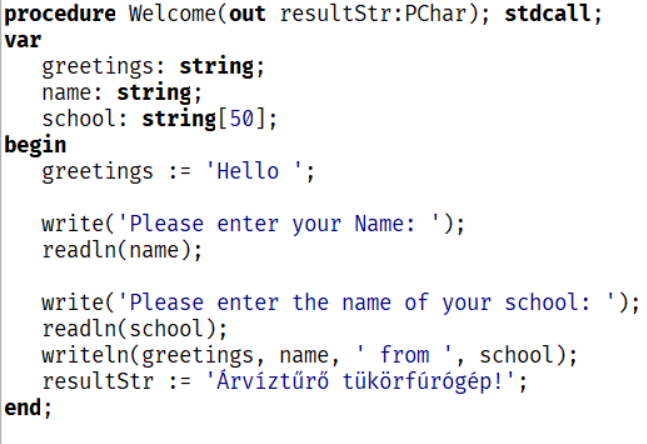
\includegraphics[scale=0.9]{hibas_string_delphi}
		\caption{Delphiben írt eljárás, amely paraméterében egy kimenő string paramétert vár.}
		\label{hibas_string_delphi}
	\end{figure}
	A C\#-ban ily módon végeztem el az eljárás deklarációját, ebben a példaprogramban ez le is futott, azonban a szakdolgozati projektünkhöz ez a megoldás nem volt megfelelő.
	\begin{figure}[h!]
		\centering
		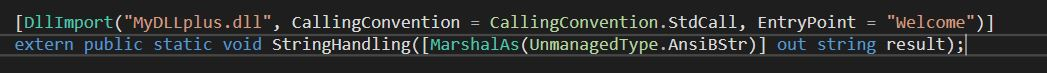
\includegraphics[scale=0.75]{hibas_string_csharp}
		\caption{Az eljárás hibás szignatúrája C\#-ban}
		\label{hibas_string_csharp}
	\end{figure}
	\subsubsection{Megoldás}
	\begin{figure}[h!]
		\centering
		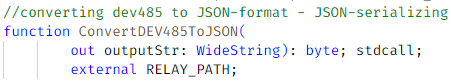
\includegraphics[scale=0.75]{string_delphi}
		\caption{A függvény helyes Delphi-deklarációja}
		\label{string_delphi}
	\end{figure}
	Stringek formájában alapértelmezetten a C\# marshalling komponense Delphiből \verb*|PWideChar| típusú változókat vár. Amennyiben Delphiben a metódus WideStringet kér paraméterben, akkor azt a C\#-oldali marshallerrel a \verb*|[MarshalAs(UnmanagedType.BStr)]| attribútum segítségével tudjuk közölni.
	\begin{figure}[h!]
		\centering
		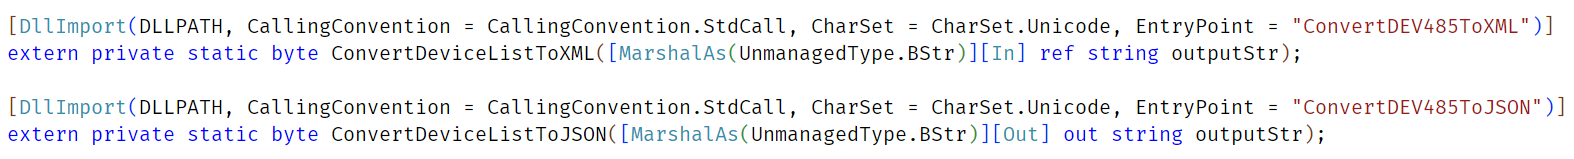
\includegraphics[scale=0.64]{string_csharp}
		\caption{A függvény helyes szignatúrája C\#-ban}
		\label{string_csharp}
	\end{figure}
	
	\cite{sof_strhandling}
	\subsection{A Delphiben eldobott kivételek nem kezelhetőek}
	\subsubsection{A probléma leírása:} Delphiben dobott kivételeket a C\# úgy érzékeli, mint hiba a külső komponensben, a tényleges kiváltó okát nem tudjuk meg.
	\subsubsection{Megoldás:} Hibakódokkal jelezzük a C\# felé, ha esetleg hibára futott valamelyik függvény, ebből a hibakódból a C\# tudni fogja, hogy milyen típusú kivételt dobjon az asztali alkalmazás számára, amelyek már lehetnek egyénileg elkészített Exception-objektumok.
	\subsection{uzfeld-metódus megfelelője C\#-ban}
	\subsubsection{A probléma leírása:} Delphiben az ablakos alkalmazásnak volt egy úgynevezett \verb*|uzfeld| nevezetű metódusa, amely a DLL üzeneteinek kezelésére szolgált, ez hívódik meg az \verb*|SLDLL_Open| meghívása után\footnote{Ez a tény, hogy a Listelem-függvény tulajdonképpen a Felmeres előtt kell, hogy meghívódjon, a Delphi7-es fejlesztői környezetének debug és breakpoint funkcióinak segítségével derült ki. Ennek használatával sorról sorra tudtam követni a program végrehajtását.} (ezért került átadásra a formot azonosító Handle). Ez azért fontos, mert az \verb*|SLDLL_Listelem|-függvény ezen az uzfeld-metóduson keresztül kerül meghívásra, a drb485 és a dev485 a program ezen pontján kapnak ténylegesen értelmezhető értékeket.
	\subsubsection{Megoldás:}
	Elméletem szerint létezik ennek egy szabványos megfelelője, C\#-ban ez \verb*|WndProc|-metódus, ami szintén Message-típusú változót vár referencia szerint átadva, ezzel tud az SLDLL futásidőben kommunikálni.
	Innentől kezdve a következő lépések játszódnak le:
	\begin{enumerate}
		\item \verb*|SLDLL_Open| kivált egy üzenetet (Win32 Message).
		\item Ezen az üzeneten keresztül az operációs rendszer meghívja a Form \verb*|WndProc| metódusát\footnote{Ezt megteheti, mivel az Open hívásakor átadott Handle révén tudja, hogy merre továbbítsa az üzeneteket.}.
		\item Amennyiben a felmérés sikeresen lezajlott, a \verb*|WndProc| meghívja a \verb*|dev485| és \verb*|drb485| változókat beállító \verb*|SLDLL_ListElem|-függvényt, mielőtt az \verb*|SLDLL_Felmeres|-re kerülne a sor. A megfelelő hívási szekvencia így automatikusan biztosított.
	\end{enumerate}
	\subsection{Eszközök azonosítóinak, típusainak átadása}
	\subsubsection{A probléma leírása:} Hogyan közöljük a felmért (USB-re csatlakoztatott) eszközök azonosítóját és típusát a C\# részére?
	\subsubsection{Megoldás:}
	A Delphiben tárolt tömb (dev485) eszközeinek legfontosabb mezőjét (ami az eszközt azonosítója, tehát az azonosítót XML-fájlba kimentjük \cite{sof_xmlcreate}, vagy JSON-formátumú szöveggé alakítjuk. Az azonosító önmagában meghatározza az eszköz típusát, úgyhogy elég azt átadni.
	Az eszközök típusát a következő módon tudjuk meghatározni kizárólag beállított azonosítóikon keresztül:
	\begin{itemize}
		\item \verb*|SLLELO|: \$4000 -> lámpa azonosítók \$4000 .. \$4fff (decimálisan: 16 384 .. 20 479) tartományon kaphatnak értéket.
		\item \verb*|SLNELO|: \$8000 -> nyíl azonosítók \$8000 .. \$8fff (decimálisan: 32 768 .. 38 683) tartományon kaphatnak értéket.
		\item \verb*|SLHELO|: \$c000 -> hangszóró azonosítók \$c000 .. \$cfff (decimálisan: 49 152 .. 53 257) tartományon kaphatnak értéket.
	\end{itemize}

	Az eszköz típusának meghatározásában nem játszik szerepet az utolsó 3 bitnégyes, tulajdonképpen a legfelső hex\footnote{4 bit azonosít egy hexadecimális számjegyet -- 0-tól F-ig terjedően --, így a bitnégyest hexnek is szokás nevezni.} azonosítja a típust.
	Szigorúan hexadecimálisan nézve: ha egy szám négyjegyű és C-számjeggyel kezdődik, akkor az azonosító hangszórót fog jelölni.

	Ez az eljárás a gRPC megoldására hasonlít, amelyet a  \ref{grpc} alfejezetben ki is fejtettem, a C\# és a Delphi között akár az XML, akár a JSON közös nyelvként (hídként) funkcionál.

	\begin{figure}[h!]
		\centering
		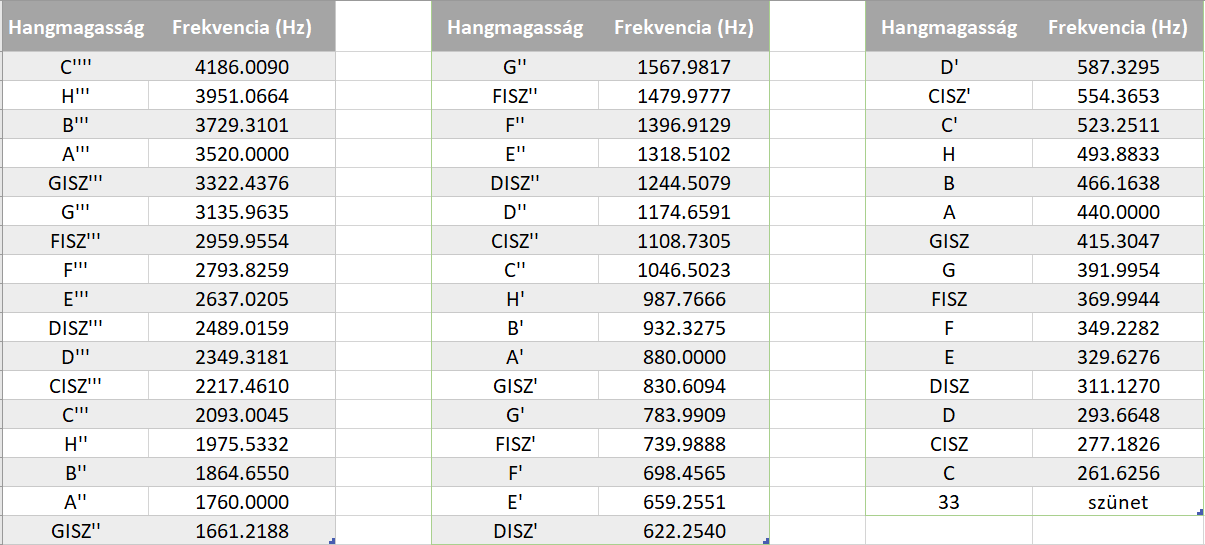
\includegraphics[scale=0.7]{frequencies}
		\caption{Hangszóróval lejátszható hangok listája}
		\subcaption{Forrás: Saját szerkesztés}
		\label{fig:frequencies}
	\end{figure}
	\section{A hangszóró egy egész hanglistát kezel - JSON}
	\subsubsection{A probléma leírása:} A hangszórók nem feltétlenül csak egy bizonyos hang, hanem egy egész hangsorozat lejátszására is képesek. Egy hang lejátszásához 3 értéket kell tudnunk:
	\begin{enumerate}
		\item index -- sorszám: Ez egy egész szám, amely egy elemre hivatkozik a frekvenciákat tartalmazó tömbből, tehát az értéke $[0;n-1]$ intervallumból kerülhet ki, ahol $n: $ a tömb hossza, esetünkben $n=50$. \ref{fig:frequencies} Ennek segítségével megadhatjuk, hogy milyen magas hangot szeretnénk a hangszóró részére lejátszásra kiküldeni.
		\item volume -- hangerő: Ez egy egész szám, amely 0 és 63 között vehet fel értéket.
		\item length -- időtartam: Szintén egész szám, amely 0 és 10000 között enged értéket beállítani az általam készített SLFormHelper DLL-ben. Ezzel megadhatjuk, hogy a hangszóró a lejátszáshoz mennyi időt vegyen igénybe, ez milliszekundumban, azaz ezredmásodperc egységben értendő.
	\end{enumerate}
	\subsubsection{Megoldás}
	Egy hanglistát több \textit{index|volume|length}-hármas ír le, a pipe, azaz '|'-karakter mentén széttördelt szövegen 3 lépésközzel iterálhatunk végig.
	\begin{figure}[h!]
		\centering
		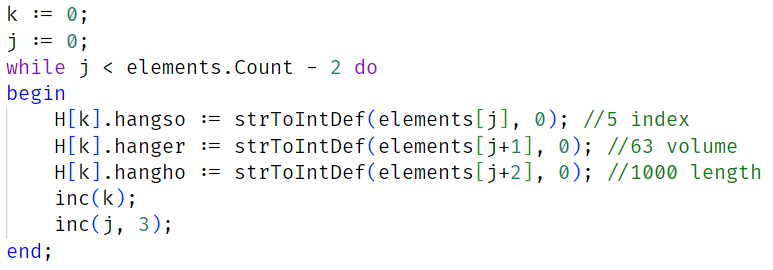
\includegraphics{speaker_solved}
		\caption{Megoldás a problémára}
		\label{speaker_solved}
	\end{figure}
	\section{A hangszóró egy egész hanglistát kezel - kód}
	\subsection{Megoldás}
	A Speaker-osztályban az eszköz viselkedését leíró 3 mezőt (index, volume és length) egy külön objektumba szervezzük ki (Sound), és a Speaker -- azonosítóján kívül -- kizárólag Sound-típusú objektumok listáját tartalmazza, a listát JSON-ben \textit{"index|volume|length"} rendezett hármasok összefűzésével szerializálja, a listához kizárólag listakezelő függvényekkel lehet hozzáférni (törlés, módosítás, hozzáadás), majd az \verb*|SLDLL_Hangkuldes| számára kiküldött H-tömböt (hanglistát) Delphiben egy ciklussal a JSON-nel átadott adatok szerint a megfelelő sorrendben feltöltjük, az előző probléma megoldásában ennek mikéntjét kifejtettem.
	%todo: ennek megoldása C#-ban
	\begin{figure}[h!]
		\centering
		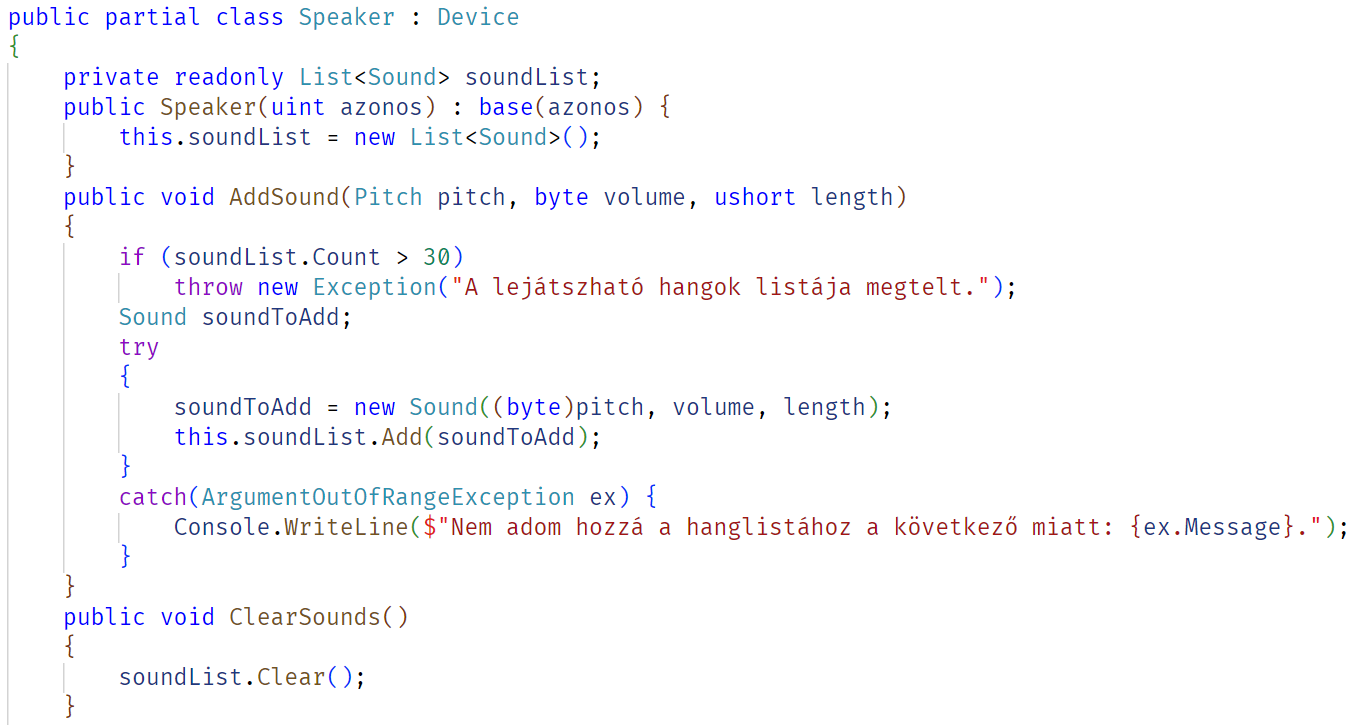
\includegraphics[scale=0.7]{speaker_csharp}
		\caption{A hangszóró hanglistát kezel - megoldás C\# nyelven}
		\label{speaker_csharp}
	\end{figure}
	\section{Két DLL működésének tesztelése}
	\cite{sof_debug_dll}
	%todo: kifejteni
	\section{Teljesítmények összehasonlítása Delphi és C\#-hívások esetében}
	\cite{sof_elapsed_time}
	
	\chapter*{Összegzés és kitekintés}
	Két ismert programozási nyelv között megteremthető kommunikáció kiaknázásával elértem, hogy egy olyan szoftver készülhessen el, amelynek segítségével szakemberek képessé válhatnak emberek mentális egészségének fejlesztésére. 
	
	Örömömre szolgált, hogy Somodi László minket bízott meg elméleteit kivitelező szoftveres háttérrel. Szakdolgozatunk nem kizárólag arról szól, hogy szakmai tudásunkat gyarapítsuk és mutassuk bizonyítványként egyetemi oktatóink felé, hanem ezzel a projekttel sok ember számára tudunk további segítséget nyújtani magunk legjobb tudása szerint.
	
	Kifejezetten tetszik, hogy munkánkat több tudományág szakértője segítette, így kutatásunk interdiszciplinárisként is jellemezhető, azaz több szakterület, jelesül a mozgáskoordináció, beágyazott rendszerek vezérlése, együttes munkájának az eredményének részesei lehettünk.
	
	A szoftverfejlesztés elméleti és gyakorlati alapjait egyrészt az Egyetem oktatóitól, szakmai és technikai vonulatait Dr. Király Roland Tanár Úrral folytatott konzultációinkon szerzett információk biztosították. 
	
	Inspirációnkat, motivációnkat Somodi Lászlóval való beszélgetéseinkből, valamint \textit{,,Mozgáskoordináció- és gyorsaságfejlesztő gyakorlatok óvodától a felnőtt korig''} címet viselő könyvében leírt gondolatokból merítettük.
	
	Mint minden szoftverre és emberi termékre jellemző, a megoldásaink természetesen nem mondhatóak tökéletesnek, programunk épp annyira időnként karbantartásra és további fejlesztésekre szorulhat. Érdekes volt felfedezni a gRPC és a Proto-nyelv kapcsán a \ref{grpc} fejezetben, hogy ötször-hatszor jobb teljesítmény érhető el az adatok bináris módon történő szerializációjával a szöveges formátumokhoz képest -- jelen állás szerint mégis az utóbbi megoldás számít elterjedtebbnek --, én azt gondolom, hogy mindenképp érdemes lenne munkánkat esetleg egy másik szakdolgozat keretein belül a gRPC irányába elmozdítani.
	\chapter*{Köszönetnyilvánítás}
	\addcontentsline{toc}{chapter}{Összegzés}
	\bibliographystyle{plain}
	\bibliography{references}
	\listoffigures
	% Aláírt, szkennelt nyilatkozat beillesztése a szakdolgozat végére
	%
\includepdf{nyilatkozat.pdf}
\end{document}